% This is file CMMP2egu.tex
%      released v1.02, 29th August 1997
%      released v1.01, 10th July 1997
% first release v1.0 beta, 5th March 1997
%   (based on CMMPguide.tex v0.35 for LaTeX2.09)
% Copyright (C) 1997 Cambridge University Press

\NeedsTeXFormat{LaTeX2e}

\documentclass{cmmp}

%%% Macros for the guide only %%%
% The following adds 6pt of space around verbatim environments.
\let\realverbatim=\verbatim
\let\realendverbatim=\endverbatim
\renewcommand\verbatim{\par\addvspace{6pt plus 2pt minus 1pt}\realverbatim}
\renewcommand\endverbatim{\realendverbatim\addvspace{6pt plus 2pt minus 1pt}}

\renewcommand\thesection{\arabic{section}}
%%% End of macros for the guide %%%


\begin{document}
\setcounter{chapter}{1}

\chapter*{\LaTeXe\ Style Guide for Authors}

\section{Introduction to \LaTeXe}

The \LaTeXe\ document preparation system is the latest version of \LaTeX\ which
is a special version of the \TeX\ typesetting program. \LaTeX\ adds to \TeX\ a
collection of commands which simplify typesetting by allowing the author to
concentrate on the logical structure of the document rather that its visual
layout.

\LaTeX\ provides a consistent and comprehensive document preparation
interface. There are simple-to-use commands for generating a table of
contents, lists of figures and/or tables, and indexes. \LaTeX\ can
automatically number list entries, equations, figures, tables, and
footnotes, as well as parts, chapters, sections and subsections. Using
this numbering system, bibliographic citations, page references and cross
references to any other numbered entity (\textit{e.g.} section, equation,
figure, list entry) are quite straightforward.

\LaTeX\ is a powerful tool for managing long and complex
documents. In particular, partial processing enables long documents
to be produced chapter by chapter without losing sequential information.

\section{The \textmd{\textsc{cmmp}} document class}

The \textsc{cmmp} document class is based on the book document class discussed
in the \LaTeXe\ manual. Commands which differ from regular \LaTeX\ or which are
in addition to regular \LaTeX\ are explained in this manual.  This short guide
is not a substitute for dedicated study of \textit{The \TeX\ book} or the
\LaTeX\ manual.

\subsection{Document class options}

In general, the standard document class options can be used, except the
following:
\begin{itemize}
\item \verb|10pt, 11pt, 12pt| --- unavailable.
\item \verb|twoside| --- \verb|twoside| is the default.
\item \verb|twocolumn| --- unavailable.
\end{itemize}
It is not advisable to use any document class options which change the way the
output looks, although most document class options can still be used without
problems.

\subsection{General}

\textbf{Warning:} There is no point spending lots of time sorting out pagination
problems with your text, as the output from CUP's \LaTeX\ may be different from
yours. Therefore it will be counter productive for the author to force lots of
pagebreaks. However this does not apply if you are producing the final camera
ready copy.

\subsection{A note on typography in this guide}

Throughout this guide, typewriter-style type will be used to indicate the
commands that you type and other characters you might see on your computer's
display screen. Braces ({\verb|{ }|}) are used to indicate \TeX's grouping
(and whenever groups are given in the definition of a command, they must be
given, even if empty [i.e., \verb|{} |], when the command is used).

\section{Installing the \textmd{\textsc{cmmp}} document class}

First, copy the \verb|cmmp.cls| file into the correct subdirectory on your hard
disk. Most implementations of \LaTeXe\ will search the current directory and
then the \verb|texinputs| directory for a class file. Therefore the best place
to store the class file is in the \verb|texinputs| directory, as this will avoid
the wrong class file being read by accident (as only one copy will exist). This
also has the advantage that any old versions of the \verb|cmmp.cls| file are
destroyed, when a new one is installed (as long as the old copy hasn't been
renamed).

\section{Starting work}

Think about the structure of the book and organise the files into manageable
pieces such as chapters. Next, create a main input file, for example,
\verb|book.tex|. This file will be set up to read in each of your input files
(\verb|chap1.tex|, \verb|chap2.tex|, \ldots, \verb|chap|\textit{n}\verb|.tex|).
Using a main input file in this way will enable you to cross-reference between
chapters and build a table of contents and index automatically. Your main input
file should look something like this:
\begin{verbatim}
\documentclass[draft]{cmmp}
\usepackage{makeidx}
\makeindex
\begin{document}
\tableofcontents

\documentclass[a4paper,11pt]{book}
%\usepackage{chapterbib}
\usepackage{dsfont}
\usepackage[title]{appendix}
\usepackage{slashbox}
\usepackage{enumerate}
\usepackage{footmisc}
%\documentclass[a4paper]{book}
% \linespread{2.}
%\numberwithin{section}
%\documentclass[12pt]{article}
%\documentclass[12pt]{cmmp}
\usepackage{textcomp}
%%\usepackage{psfig}
%\usepackage{harvard}
\usepackage{epsfig}
\usepackage{amsmath}   
\usepackage{amsfonts}
%\counterwithin{figure}{section}
\usepackage{amssymb}
\usepackage{bbold}
\usepackage{bbm}
\numberwithin{equation}{section}
\numberwithin{figure}{section}
\numberwithin{table}{section}
%%\usepackage{graphicx}
%%
%%\usepackage{txfonts}
%%%\usepackage{mathrsfs}
%
%%\usepackage{feynmf}     %<------------ Obbligatorio
\unitlength=1mm         %<------------ Obbligatorio
%
\newsavebox{\fmbox}
\newenvironment{fmpage}[1]
{\begin{lrbox}{\fmbox}\begin{minipage}{#1}}
{\end{minipage}\end{lrbox}\fbox{\usebox{\fmbox}}}
\newcommand{\braket}[1]{\langle {#1} \rangle }
\newcommand{\ket}[1]{|{#1} \rangle }
\newcommand{\bra}[1]{\langle {#1}|}
\newcommand\idop{\mathds 1}
\usepackage{dsfont}
\usepackage{latexsym}
\usepackage[varg]{txfonts}
\usepackage{mathrsfs}
\usepackage{upgreek}
\usepackage[round]{natbib}
%\usepackage [latin1]{inputenc}
\usepackage{verbatim}
\usepackage{array}
\usepackage{color}
%\pagestyle{plain}
\usepackage{graphicx}
\usepackage{caption}
\DeclareMathAlphabet{\mathpzc}{OT1}{pzc}{m}{it}
\begin{document}
\section{Views of the nucleus}
In the atom, the nucleus provides the Coulomb field in which negatively charged electrons $(-1\times e)$ move indenpendently of each other in single--particle orbitals. The filling of these orbitals explains Mendeleev's periodic table. Thus the valence of the chemical elements as well as the particular stability of the noble gases (He, N, Ar, Kr, Xe and Ra) associated with the closing of shells (Fig. \ref{fig1.0.1}). The dimension of the atom is measured in angstroms (\AA=$10^{-8}$cm), and typical energies in eV, the electron mass being $m_e\approx 0.5$ MeV (MeV=$10^6$eV).


The atomic nucleus is made out of positively charged protons ($1\times e$) and of (uncharged) neutrons, nucleons, of mass $\approx 10^3$ MeV ($m_p=938.3$ MeV, $m_n=939.6$ MeV). Nuclear dimensions are of the order of few fermis (fm$=10^{-13}$ cm). While the stability of the atom is provided by a source external to the electrons, namely the atomic nucleus, this system is  self--bound as a result of the strong interaction of range $a_0\approx 0.9$ fm and strength $v_0\approx -100$ MeV acting among nucleons. 
\subsection{The liquid drop and the shell model}
While most of the atom is empty space, the density of the atomic nucleus is conspicuous ($\rho=0.17$ nucleon/fm$^3$). The ``closed packed'' nature of this system implies a short mean free path as compared to nuclear dimensions. This can be estimated from classical kinetic theory $\lambda\approx(\rho\sigma)^{-1}\approx1$ fm, where $\sigma\approx 2\pi a_0^2$ is the nucleon--nucleon cross section. It seems then natural to liken the atomic nucleus to a liquid drop (Bohr and Kalckar).
This picture of the nucleus provided the framework to describe the basic features of the fission process (\cite{Meitner:39,Bohr:39}). 



The leptodermic properties of the atomic nucleus are closely connected with the semi--empirical mass formula (\cite{Weizsacker:35})
\begin{align}
m(N,Z)=(Nm_n+Zm_p)-\frac{1}{c^2}B(N,Z),
\end{align}
the binding energy being
\begin{align}\label{eq1.0.2}
B(N,Z)=\left(b_{vol}A-b_{surf}A^{2/3}-\frac{1}{2} b_{sym}\frac{(N-Z)^2}{A}-\frac{3}{5}\frac{Z^2e^2}{R_C}\right).
\end{align}
The second term in (\ref{eq1.0.2}) represents the surface energy, while
\begin{align}\label{eq1.0.3}
b_{surf}=4\pi r_0^2\gamma.
\end{align}
The nuclear radius is written as $R=r_0A^{1/3}$, with $r_0=1.2$ fm, the surface tension energy being $\gamma\approx 0.95$ MeV/fm$^2$.


When, in a heavy--ion reaction,  two nuclei come within the range of the nuclear forces, the trajectory of relative motion will be changed by the attraction which will act between the nuclear surfaces. This surface interaction is a fundamental quantity in all heavy ion reactions. Assuming two spherical nuclei at a relative distance $r_{aA}=R_a+R_A$, where $R_a$ and $R_A$ are the corresponding half--density radii, the force acting between the two surfaces is
\begin{align}\label{eq1.0.4}
\left(\frac{\partial U_{aA}^N}{\partial r}\right)_{r_{aA}}=4\pi \gamma\frac{R_aR_A}{R_a+R_A}
\end{align}
This result allows for the calculation of the ion--ion (proximity) potential which, supplemented with a position dependent absorption, can be used to accurately describe heavy ion reactions\footnote{\cite{Broglia:04a} and refs. therein.}.


In such reactions, not only elastic processes are observed, but also anelastic processes in which one, or both of the nuclear surfaces is set into vibration (Fig. \ref{fig1.0.2}). The restoring force parameter associated with oscillations of multipolarity $\lambda$ is 
\begin{align}\label{eq1.0.4b}
C_\lambda=(\lambda-1)(\lambda+2)R^2\gamma-\frac{3}{2\pi}\frac{\lambda-1}{2\lambda+1}\frac{Z^2e^2}{R},
\end{align}
where the second term corresponds to the contribution of the Coulomb energy to $C_\lambda$. Assuming the flow associated with surface vibration to be irrotational, the associated inertia for small amplitude oscillations is, 
\begin{align}\label{eq1.0.5}
D_{\lambda}=\frac{3}{4\pi}\frac{1}{\lambda}AMR^2,
\end{align}
the energy of the corresponding mode being
\begin{align}\label{eq1.0.6}
\hbar\omega_\lambda=\hbar\sqrt{\frac{C_\lambda}{D_\lambda}}.
\end{align}
The label $\lambda$ stands for the angular momentum of the vibrational mode, $\mu$ being its third component (see Eq. (\ref{eq1.0.12})). Aside from $\lambda,\mu$, surface vibrations can also be characterized by an integer $n(=1,2,\dots)$, an ordering number indicating increasing energy. For simplicity, a single common label $\alpha$ will be also used.


Experimental information associated with low--energy quadrupole vibrations, namely $\hbar\omega_{2}$ and the electromagnetic transition probabilities $B(E2)$, allow to determine $C_2$ and $D_2$. The resulting $C_2$ values exhibit variations by more than a factor of 10 both above and below the liquid--drop estimate. The observed values of $D_2$ are large as compared with the mass parameter for irrotational flow.

A picture apparently antithetic to that of the liquid drop, the shell model, emerged from the study of experimental data, plotting them against either the number of protons (atomic number), or the number of neutrons in the nuclei, rather than against the mass number.
One of the main nuclear features which led to the development of the shell model was the study of the stability and abundance of nuclear species and the discovery of what are usually called magic numbers (\cite{Elsasser:33,Mayer:48,Haxel:49}). What makes a number magic is that a configuration of a magic number of neutrons, or of protons, is unusually stable whatever the associated number of other nucleons (\cite{Mayer:49,Mayer:49b}).


The strong binding of a magic number of nucleons and weak binding for one more reminds, only relatively much weaker, the results displayed in Fig.  \ref{fig1.0.1}  concerning the atomic stability o\bibliographystyle{abbrvnat}f rare gases. In the nuclear case, at variance with the atomic case, the spin--orbit coupling play an important role, as can be seen from the level scheme shown in Fig. \ref{fig1.0.3}, obtained by assuming that nucleons move independently of each other in an average potential  of  spherical symmetry.


A closed shell, or a filled level, has angular momentum zero. Thus, nuclei with one nucleon outside (missing from) closed shell, should have the spin and parity of the orbital associated with the odd nucleon (--hole), a prediction confirmed by the data (available at that time) throughout the mass table. Such a picture implies that the nucleon mean free path is large compared to nuclear dimensions.


The systematic studies of the binding energies leading to the shell model found also that formula (\ref{eq1.0.2}) has to be supplemented to take into account the fact that nuclei with both odd number of protons and of neutrons are energetically unfavored compared with even--even ones (inset Fig. \ref{fig1.0.1}) by a quantity of the order of $\delta\approx33MeV/A^{3/4}$ called the pairing energy\footnote{Connecting with further developments associated with the BCS theory of superconductivity (\cite{Bardeen:57a,Bardeen:57b}) and its extension to the atomic nucleus (\cite{Bohr:58}), the quantity $\delta$ is identified with the pairing gap $\Delta$ parametrized according to $\Delta=12 $MeV$/\sqrt{A}$ (\cite{Bohr:69}). It is of notice that for typical superfluid nuclei like $^{120}$Sn, the expression of $\delta$ leads to a numerical value which can be parametrized as  $\delta\approx10$ MeV$/\sqrt{A}$.}.

The low--lying excited state of closed shell nuclei can be interpreted as a rule, as harmonic quadrupole or octupole collective vibrations (Fig. \ref{fig1.0.4}) described by the Hamiltonian\footnote{Classically $\Pi_{\lambda\mu}=D_\lambda\dot\alpha_{\lambda\mu}$.}
\begin{align}\label{eq1.0.7}
H_{coll}=\sum_{\lambda\mu}\left(\frac{1}{2D_{\lambda}}|\Pi_{\lambda\mu}|^2+\frac{C_\lambda}{2}|\alpha_{\lambda\mu}|^2\right)
\end{align}
Following \cite{Dirac:26} one can describe the oscillatory motion introducing boson creation (annihilation) operator $\Gamma_{\lambda\mu}^\dagger$ ($\Gamma_{\lambda\mu}$) obeying
\begin{align}\label{eq1.0.8}
\left[\Gamma_{\alpha},\Gamma_{\alpha'}^\dagger\right]=\delta(\alpha,\alpha'),
\end{align}
leading to 
\begin{align}\label{eq1.0.9}
\hat\alpha_{\lambda\mu}=\sqrt{\frac{\hbar\omega_\lambda}{2C_\lambda}}\left(\Gamma_{\lambda\mu}^\dagger+(-1)^\mu\Gamma_{\lambda-\mu}\right),
\end{align}
and a similar expression for the conjugate momentum variable $\hat\Pi_{\lambda\mu}$, resulting in 
\begin{align}\label{eq1.0.9b}
\hat H_{coll}=\sum\hbar\omega_\lambda\left((-1)^\mu\Gamma_{\lambda\mu}^\dagger\Gamma_{\lambda-\mu}+1/2\right).
\end{align}
The frequency is $\omega_\lambda=(C_\lambda/D_\lambda)^{1/2}$, while $(\hbar\omega_\lambda/2C_\lambda)^{1/2}$ is the amplitude of the zero--point fluctuation of the vacuum state $\ket{0}_B,\ket{n_{\lambda\mu}=1}\Gamma_{\lambda\mu}^\dagger \ket{0}_B$ being the one--phonon state. To simplify the notation, in many cases one writes $\ket{n_\alpha=1}$.

The ground and low--lying states of nuclei with one nucleon outside closed shell can be described by the Hamiltonian
\begin{align}\label{eq1.0.10}
H_{sp}=\sum_{\nu}\epsilon_\nu a_\nu^\dagger a_\nu,
\end{align}
where $a_\nu^\dagger (a_\nu)$ is the single--particle creation (annihilation) operator,
\begin{align}\label{eq1.0.11}
\ket{\nu}=a_\nu^\dagger\ket{0}_F,
\end{align}
being the single--particle state of quantum numbers $\nu(\equiv nljm)$ and energy $\epsilon_\nu,\ket{0}_F$ being the Fermion vacuum. 
It is of notice that
\begin{align}\label{eq0.1.14}
\left[H_{coll},\Gamma^\dagger_{\lambda'\mu'}\right]=\hbar\omega_{\lambda'}\Gamma^\dagger_{\lambda'\mu'}
\end{align}
and 
\begin{align}\label{eq0.1.15}
\left[H_{sp},a^\dagger_{\nu'}\right]=\epsilon_{\nu'}a^\dagger_{\nu'}.
\end{align}
	This is an obvious outcome resulting from the bosonic
\begin{align}
\left[\Gamma_{\alpha},\Gamma^\dagger_{\alpha'}\right]=\delta(\alpha,\alpha')
\end{align}
	and fermionic
\begin{align}
\left\{a_\nu,a^\dagger_{\nu'}\right\}=\delta(\nu,\nu')
\end{align}
commutation relations.
Both the existence of drops of nuclear matter displaying collective surface vibrations, and of independent--particle motion in a self--confining mean field are emergent properties not contained in the particles forming the system, neither in the $NN$--force, but on the fact that these particles behave according to the rules of quantum mechanics, move in a confined volume and that there are many of them.


Generalized rigidity as measured by the inertia parameter $D_\lambda$, as well as surface tension closely connected to the restoring force $C_\lambda$, implies that acting on the system with an external time--dependent (nuclear and/or Coulomb) field, the system reacts as a whole. This behavior is to be found nowhere in the properties of the nucleons, nor in the nucleon--nucleon scattering phase shifts at the basis of Yukawa prediction of the existence of a $\pi$--meson as the carrier of the strong force acting among nucleons.


Similarly, the fact that nuclei probed through fields which change in one unit particle number (e.g. $(d,p)$ and $(p,d)$ reactions) react in term of independent particle motion,  feeling the pushings and pullings of the other nucleons only when trying to leave the nucleus, is not apparent in the detailed properties of the $NN$--forces, not even in those carrying the quark--gluon input. Within this context, independent particle motion can be considered a \textit{bona fide} emergent property.


Collective surface vibrations and independent particle motion are examples of what are called elementary modes of excitation in many--body physics, and collective variables in soft--matter physics.
\section{The particle-vibration coupling}
The oscillation of the nucleus under the influence of surface tension implies that the potential $U(R,r)$ in which nucleons move independently of each other change with time. For low--energy collective vibrations this change is slow as compared with single--particle motion. Within this scenario the nuclear radius can be written as  
\begin{align}\label{eq1.0.12}
R=R_0\left(1+\sum_{LM}\alpha_{\lambda\mu}Y_{\lambda\mu}^*(\hat r)\right)
\end{align}
Assuming small amplitude motion,
\begin{align}\label{eq1.0.13}
U(r,R)=U(r,R_0)+\delta U(r),
\end{align}
where
\begin{align}\label{eq1.0.14}
\delta U=-\kappa\hat \alpha \hat F,
\end{align}
and
\begin{align}\label{eq1.0.15}
\hat F=\sum_{\nu_1\nu_2}\bra{\nu_1}F\ket{\nu_2}a_{\nu_1}^\dagger a_{\nu_2},
\end{align}
while
\begin{align}\label{eq1.0.16}
F=\frac{R_0}{\kappa}\frac{\partial U}{\partial r}Y^*_{\lambda\mu}(\hat r).
\end{align}
The coupling between surface oscillation and single--particle motion, namely the particle vibration coupling (PVC) Hamiltonian $\delta U$ (Fig. \ref{fig1.0.5}) is a consequence of the overcompleteness of the basis. Diagonalizing $\delta U$ making use of the graphical (Feynman) rules of Nuclear Field Theory (NFT) to be discussed in following Chapter, one obtains structure results which can be used in the calculation of transition probabilities and reaction cross sections, quantities which can be compared with experimental findings.

  
In fact, within the framework of NFT, single--particles are to be calculated as the Hartree--Fock solution of the $NN$--interaction $v(|\mathbf r-\mathbf r'|)$ (Fig. \ref{fig1.0.6}), in particular
\begin{align}\label{eq1.0.18}
U(r)=\int d\mathbf r' \rho(r')v(|\mathbf r-\mathbf r'|
\end{align}
being the Hartree field\footnote{To this potential one has to add the Fock potential resulting from the fact that nucleons are fermions. This exchange potential (Fig. \ref{fig1.0.6} (2 and 4)) is essential in the determination of single--particle energies and wavefunctions. Among other things, it takes care of eliminating the nucleon self interaction from the Hartree field.} expressing the selfconsistency between density $\rho$ and potential $U$ (Fig. \ref{fig1.0.6} (b) (1) and (3)), while vibrations are to be calculated in the Random Phase Approximation (RPA) making use of the same interaction\footnote{The sum of the so called ladder diagrams (see Fig. \ref{fig1.0.7}) are taken into account to infinite order in RPA. This is the reason why bubble contributions in the diagonalization of Eq. \ref{eq1.0.19b} are not allowed in NFT, being already contained in the basis states.} (Fig. \ref{fig1.0.7}), extending the selfconsistency to fluctuations $\delta\rho$ of the density and $\delta U$ of the mean field, that is,
\begin{align}\label{eq1.0.19}
\delta U(r)=\int d\mathbf r' \delta \rho(r')v(|\mathbf r-\mathbf r'|.
\end{align}
Making use of the  solution of the selfconsistent relation (\ref{eq1.0.19}), one obtains the transition density $\delta\rho$. The matrix elements $\braket{n_\lambda=1, \nu_i|\delta\rho|\nu_k}$ provide the  particle--vibration coupling strength to work out the variety of coupling processes between single--particle and collective motion (Fig. \ref{fig1.0.5}). That is, the matrix element of the PVC Hamiltonian $H_c$. Diagonalizing 
\begin{align}\label{eq1.0.19b}
H=H_{HF}+H_{RPA}+H_c+v,
\end{align}
applying  in the basis of single--particle and collective modes, that is solutions of $H_{HF}$ and of $H_{RPA}$ respectively, the  NFT rules   one obtains a solution of the total Hamiltonian. Concerning the rules of NFT, they codify the way in which $H_c$ and $v$ are to be treated to all orders of perturbation theory. Also which processes (diagrams) are not allowed because they will imply overcounting of correlations already included in the basis states\footnote{A simple, although not directly related but only in a general way, example is provided by Eq. (2A-31) of \cite{Bohr:69} i.e. $G=\tfrac{1}{4}\sum_{\nu_1\nu_2\nu_3\nu_4}\braket{\nu_3\nu_4|G|\nu_1\nu_2}_ aa^\dagger(\nu_4)a^\dagger(\nu_3)a(\nu_1)a(\nu_2)=\tfrac{1}{2}\sum_{\nu_1\nu_2\nu_3\nu_4}\braket{\nu_3\nu_4|G|\nu_1\nu_2} a^\dagger(\nu_4)a^\dagger(\nu_3)a(\nu_1)a(\nu_2)$ where $\braket{\;}_a$ is the antisymmetric matrix element.} (single-particle HF, collective vibrations, RPA). 


Because of quantal zero point fluctuations, a nucleon propagating in the nuclear medium moves through a cloud of bosonic and fermionic virtual excitations to which it couples ($H_c+v$), becoming dressed and acquiring an effective mass, charge, etc. (Fig. \ref{fig1.0.8}). Vice versa, vibrational modes can become renormalized through the coupling to dressed nucleons which, in intermediate virtual states, can exchange the vibrations which produce their clothing, with the second fermion (hole state). Such a process leads to a renormalization of the PVC vertex\footnote{It is to be noted that in the case in which the renormalized vibrational modes, i.e. the initial and final wavy lines in Fig. \ref{fig1.0.4} have angular momentum and parity $\lambda^\pi=0^+$, and one uses a model in which there is symmetry between the particle and the hole subspaces, the four diagrams sum to zero, because of particle conservation.} (Fig. \ref{fig1.0.5}) (\cite{Bertsch:83,Barranco:04} and refs. therein), as well as of the bare $NN$--interaction. 

An alternative procedure to the diagramatic one to obtain the HF and RPA solutions associated with the bare $NN$-interaction $v$ is provided by the relations (\ref{eq0.1.15}) and (\ref{eq0.1.14}) respectively, replacing the Hamiltonians by $(T+v)$, where $T$ is the kinetic energy operator. The phonon operator associated with surface vibrations is defined through
\begin{align}\label{eq1.0.26}
\Gamma_\alpha^\dagger=\sum_{ki}X_{ki}^\alpha\Gamma_{ki}^\dagger+Y_{ki}^\alpha\Gamma_{ki},
\end{align}
and the normalization condition 
\begin{align}\label{eq1.0.27}
\left[\Gamma_\alpha,\Gamma_\alpha^\dagger\right]=\sum_{ki}\left(X_{ki}^{\alpha2}+Y_{ki}^{\alpha2}\right)=1.
\end{align}
The operator $\Gamma^\dagger_{ki}=a^\dagger_{k}a_{i} (\epsilon_k>\epsilon_F,\epsilon_i<\epsilon_F)$ creates a particle-hole excitation acting on the HF vacuum state $\ket{0}_F$. It is assumed that
\begin{align}\label{eq1.0.28}
\left[\Gamma_{ki},\Gamma_{k'i'}^\dagger\right]=\delta(k,k')\delta(i,i').
\end{align}
Within this context, RPA is a harmonic, quasi-boson approximation.


From being antithetic views of the nuclear structure, a proper analysis of the experimental data testifies to the fact that the collective and the independent particle pictures of the nuclear structure require and support each other (\cite{Bohr:75}). To obtain a quantitative description of nucleon  motion and nuclear phonons (vibrations), one needs a proper description of the $k$-- and $\omega$--dependent ``dielectric'' function of the nuclear medium, in a similar way in which a proper description of the reaction processes used as probes of the nuclear structure requires the use of the optical potential (continuum ``dielectric'' function). The NFT solution of (\ref{eq1.0.19b}) provide all the elements to calculate the  structure properties of nuclei, and also  the optical potential needed to describe nucleon--nucleus scattering and reaction processes. It furthermore shows that both single--particle and vibrational elementary modes of excitation emerge from the same properties of the $NN$--interaction. The question of relating it in a direct fashion with the absolute differential cross sections (observables) remains open, in keeping with the important role played by the many-body renormalization processes and associated emergent properties.


The development of experimental techniques and associated hardware has allowed for the identification of a rich variety of elementary modes of excitation aside from collective surface vibrations and of independent particle motion: quadrupole and octupole rotational bands, giant resonance of varied multipolarity and isospin, as well as pairing vibrations and rotation, together with giant pairing vibrations of transfer quantum number $\beta\pm 2$. Modes which can be specifically excited in inelastic and Coulomb excitation processes, and one- and two-particle transfer reactions.
\section{Pairing vibrations}
Let us introduce this new type of elementary mode of excitation by making a parallel with quadrupole surface vibrations within the framework of RPA, namely
\begin{align}\label{eq1.0.29}
\left[(H_{sp}+H_i),\Gamma_{k'i'}^\dagger\right]=\hbar\omega_\alpha\Gamma_{k'i'}^\dagger,
\end{align}
where for simplicity we use, instead of $v$, a quadrupole-quadrupole separable interaction $(i=QQ)$ defined as
\begin{align}\label{eq1.0.30}
H_{QQ}=-\kappa\hat Q^\dagger Q
\end{align}
with 
\begin{align}\label{eq1.0.31}
\hat Q^\dagger=\sum_{ki}\braket{k|r^2 Y_{2\mu}|i}a^\dagger_k a_i,
\end{align}
while $H_{sp}$ and $\Gamma^\dagger_\alpha$ are defined in (\ref{eq1.0.10}) and (\ref{eq1.0.26}) supplemented by (\ref{eq1.0.27}).

In connection with the pairing energy mentioned in relation with the inset of Fig. \ref{fig1.0.1}, it is a consequence of correlation of pairs of like nucleons moving in time reversal states. A similar phenomenon found in metals at low temperatures and giving rise to superconductivity. The pairing interaction $(i=P)$ can be written, within the approximation (\ref{eq1.0.30}) used in the case of the quadrupole-quadrupole force as 
\begin{align}\label{eq1.0.32}
H_P=-\hat P^\dagger P,
\end{align}
where 
\begin{align}\label{eq1.0.33}
\hat P^\dagger=\sum_{\nu>0}a^\dagger_\nu a^\dagger_{\bar\nu}.
\end{align}
Consequently, in this case the concept of independent particle field $\hat Q$ (see also (\ref{eq1.0.15})) associated with particle-hole ($ph$) excitations and carrying transfer quantum number $\beta=0$ has to be generalized to include fields describing independent pair motion, in which case $\alpha\equiv(\beta=+2,J^\pi=0^+)$
\begin{align}\label{eq1.0.34}
\Gamma^\dagger_\alpha=\sum_kX^\alpha_{kk}\Gamma_k^\dagger+\sum_iY^\alpha_{ii}\Gamma_i
\end{align}
with 
\begin{align}\label{eq1.0.35}
\Gamma^\dagger_k=a^\dagger_ka^\dagger_{\bar k}\;(\epsilon_k>\epsilon_F),\quad \Gamma^\dagger_i=a^\dagger_ia^\dagger_{\bar i}\;(\epsilon_i<\epsilon_F),
\end{align}
and
\begin{align}\label{eq1.0.36}
\sum_kX_{kk}^{\alpha 2}-\sum_i Y_{ii}^{\alpha 2}=1
\end{align}
for the pair addition ($(pp),\beta=+2$) mode, and a similar expression for the pair removal ($(hh),\beta=-2$) mode. In Fig. \ref{fig1.0.3} the NFT graphical representation of the RPA equations for the pair addition mode is given. The state $\Gamma^\dagger_\alpha(\beta=+2)\ket{\tilde 0}$, where $\ket{\tilde 0}$ is the correlated ground state of a closed shell nucleus, can be viewed as the nuclear embodiment of a Cooper pair found at the basis of the microscopic theory of superconductivity.


While surface vibrations are associated with the normal $(\beta=0)$ nuclear density, pairing vibrations are connected with the\dots

Similarly to the quadrupole and octupole vibrational bands built out of $n_\alpha$ phonons of quantum numbers $\alpha\equiv(\beta=0,\lambda^\pi=2^+,3^-)$ schematically shown in Fig. \ref{fig1.0.4} and experimentally observed in inelastic and Coulomb excitation and associated $\gamma$-decay processes, pairing vibrational bands build of $n_\alpha$ phonons of quantum numbers $\alpha\equiv(\beta=\pm2,\lambda^\pi=0^+,2^+)$ have been identified around closed shells in terms of nucleon-transfer reactions throughout the mass table (Fig. \ref{fig1.0.}).
\section{Spontaneous broken symmetry}
Because empty space is homogeneous and isotropic, the nuclear Hamiltonian is translational and rotational invariant. It also conserves particle number and is thus gauge invariant. According to quantum mechanics, the corresponding wavefunctions transform in an irreducible way under the corresponding group of transformations.

When the solution  of the Hamiltonian does not have some of these symmetries, for example defines a privileged direction in space violating rotational invariance, one is confronted with the phenomenon of spontaneous broken symmetry. Strictly \dots for idealized systems that are infinitely large
\subsection{Quadrupole deformations in 3D-space}
A nuclear embodiment of the spontaneous symmetry breaking phenomenon is provided by a quadrupole deformed  mean field. A situation one is confronted with, when the value of the lowest quadrupole frequency $\omega_2$ of the RPA solution (\ref{0.1.14}) (see also (\ref{0.1.26}) and (\ref{0.1.27})) tends to zero ($C_2\to0$, $D_2$ finite). A phenomenon resulting from the interplay of the interaction $v$ ($H_QQ$ in (\ref{0.1.29})), and of the nucleons outside closed shell, leading to tidal-like polarization of the spherical core.

Coordinate and linear momentum (($x,p_x$) single-particle motion) as well as Euler angles and angular momentum (($\varphi,I_z$) rotational two-dimensional (2D)-space) are conjugate variables. Similarly, the gauge angle and the number of particles (($\phi,N$) rotation in gauge space), fulfill $[\phi,N]=i$. The operators $e^{-ip_xx}$, $e^{-i\varphi I_z}$ and $e^{-iN\phi}$ induce Galilean transformation and rotations in 2D- and in gauge space respectively.

Making again use, for didactical purposes, of $H_{QQ}$ instead of $v$, and calling $\ket{N}$ the eventual mean field solution of the Hamiltonian $T+H_{QQ}$, one expects
  \begin{align}\label{eq0.4.1}
\braket{N|\hat Q|N}=Q_0,
  \end{align}
where, for simplicity, we assumed axial symmetry $(\lambda=2,\mu=0)$. That is, the emergence of a static quadrupole deformation.
Rewriting $H_{QQ}$ in terms of $(\hat Q^\dagger-Q_0+Q_0)$ and its Hermitian conjugate, one obtains 
  \begin{align}\label{eq0.4.2}
H=H_{sp}+H_{QQ}=H_{MF}+H_{fluct},
\end{align}
where 
  \begin{align}\label{eq0.4.3}
H=H_{MF}=H_{sp}-\kappa(\hat Q^\dagger+\hat Q),
\end{align}
is the mean field, and
\begin{align}\label{eq0.4.4}
H_{fluct}=-\kappa(\hat Q^\dagger-Q_0)(\hat Q-Q_0)
\end{align}
the residual interaction inducing fluctuations around $Q_0$. Assuming $Q_0\gg (\hat Q^\dagger-Q_0)(\hat Q-Q_0)$, we concentrate on $H_{MF}$. The original realization of it is known as the Nilsson Hamiltonian (\cite{Nilsson:55}). It describes the motion of nucleons in a single-particle potential of radius $R_0(1+\beta_2Y_{20}(\hat r))$, with $\beta_2$ proportional to the intrinsic quadrupole \dots The reflection invariance and axial symmetry of the Nilsson Hamiltonian implies that parity $\pi$ and projection $\Omega$ of the total angular momentum along the symmetry axis are constants of motion for the one-particle Nilsson states. These states, are two-fold degenerate, since two orbits that differ only in the sign of $\Omega$ represent the same motion, appart from the clockwise and anticlockwise sense of revolution around the symmetry axis. One can thus write the Nilsson creation operators in terms of a linear combination of creation operators carrying good total angular momentum $j$, 
\begin{align}\label{eq0.4.5}
\gamma^\dagger_{a\Omega}=\sum_jA_j^aa^\dagger_{aj\Omega},
\end{align}
where the label $a$ stands for all the quantum numbers aside from $\Omega$, which specify the orbital. 

Expressed in the intrinsic, body-fixed, system of coordinates $\mathcal K'$ where the 3 ($z'$) axis lies along the symmetry axis and the 1 and 2 ($x',y'$) axis lie in a plane perpendicular to it, namely
\begin{align}\label{eq0.4.6}
\gamma'^{\dagger}_{a\Omega}=\sum_jA_j^a\sum_{\Omega'}\mathcal D_{\Omega\Omega'}^2(\omega)a^\dagger_{aj\Omega'},
\end{align}
one can write the Nilsson state as 
\begin{align}\label{eq0.4.7}
\ket{N(\omega)}_{\mathcal K'}=\prod_{a\Omega>0}\gamma'^{\dagger}_{a\Omega}\gamma'^{\dagger}_{a\widetilde\Omega}\ket{0}_F,
\end{align}
where $\omega$ represent the Euler angles, $\ket{0}_F$ is the particle vacuum, and $\ket{a\widetilde\Omega}=\gamma'^{\dagger}_{a\widetilde\Omega}\ket{0}_F$ is the state time-reversed to $\ket{a\Omega}$. For well deformed nuclei, a conventional description of the one-particle motion is based on the similarity of the nuclear potential to that of an anisotropic nuclear potential, 
\begin{align}\label{eq0.4.8}
V=\frac{1}{2}M\left(\omega_3^2x_3^2+\omega^2_{\perp}(x_1^2+x_x^2)\right)=\frac{1}{2}M\omega_0r^2\left(1-\frac{4}{3}\delta P_2(\cos\theta)\right),
\end{align}
with $\omega_3\omega_{\perp}^2=\omega_0^3$. That is a volume which is independent of the deformation $\delta\approx0.95\beta_2$. The corresponding single-particle states have energy
\begin{align}\label{eq0.4.9}
\epsilon(n_3n_{\perp})=(n_3+\tfrac{1}{2})\hbar\omega_3+(n_{\perp}+\tfrac{1}{2})\hbar\omega_{\perp},
\end{align}
where $n_3$ and $n_{\perp}=n_1+n_2$ are the number of quanta along and perpendicular to the symmetry axis. The degenerate states with the same value of $n_{\perp}$ can be specified by the component $\Lambda$\dots symmetry axis,
\begin{align}\label{eq0.4.10}
\Lambda=\pm n_{\perp}, \pm(n_{\perp}-2),\dots,\pm 1\text{ or } 0.
\end{align}
One can then label the Nilsson levels in terms of the asymptotic quantum numbers $[Nn_3\Lambda\Omega]$, where $N=n_3+n_{\perp}$, is the total oscillator quantum number.

The complete expression of the Nilsson potential includes, aside from the central term discussed above, a spin-orbit and a term proportional to the orbital angular momentum quantity squared, so as to make the shape of the oscillator to resemble more that of a Saxon-Woods potential. The resulting levels provide an overall account of the experimental findings, providing detailed evidence in terms of individual states of the interplay between the single-particle and the collective aspects of nuclear structure. An example of relevance for light nuclei ($N$ and $Z<20$) is given in Fig. \ref{fff}.

The Nilsson intrinsic state (\ref{eq0.4.7}) does not have a definite angular momentum but is rather a superposition of such states,
\begin{align}\label{eq0.4.11}
\ket{N(\omega)}_{\mathcal K'}=\sum C_I\ket{I}.
\end{align}
Because there is no restoring force associated with different orientations of $\ket{N(\omega}_{\mathcal K'}$, fluctuations in the Euler angle diverge in the right way to restore rotational invariance, leading to a rotational band whose members are 
\begin{align}\label{eq0.1.47}
\ket{IKM}\sim\int d\omega \,\mathcal D^I_{MK}(\omega)\,\ket{N(\omega)}_{\mathcal K'},
\end{align}
with energy
\begin{align}\label{eq0.1.48}
E_I=\frac{\hbar^2}{2\mathcal I}I(I+1).
\end{align}
The quantum numbers $I,M,K$ are the total angular momentum $I$, and its third component $M$ and $K$ along the laboratory ($z$) and intrinsic ($z'$) frame references respectively.


Rotational bands have been observed up to rather high angular momenta in terms of individual transitions. An example extending up to $I=60\hbar$ is given in Fig. \ref{0.4.2}. 
\subsection{Deformation in gauge space}
Let us now turn to the airing Hamiltonian. In the case in which $\hbar\omega_{\beta=-2}\approx0$, the system deforms, this time in gauge space. Calling $\ket{BCS}$ the eventual mean field value leads to a finite value \dots of the pair operator $P^\dagger$ which can be viewed as the order parameter of the new (gauge deformed) phase of the system. The total Hamiltonian can be written as
\begin{align}\label{eq0.1.50}
H=H_{MF}+H_{fluct},
\end{align}
where 
\begin{align}\label{eq0.1.51}
H_{MF}=H_{sp}-\Delta(P^\dagger+P)+\frac{\Delta^2}{G}
\end{align}
and
\begin{align}\label{eq0.1.52}
H_{fluct}=-G(P^\dagger-\alpha_0)(P-\alpha_0).
\end{align}
The quantity 
\begin{align}\label{eq0.1.53}
\Delta=G\alpha_0
\end{align}
is the so called pairing gap, which measures the binding energy of Cooper pairs, $\alpha_0$ counting the number of Cooper pairs. The mean field pairing Hamiltonian 
\begin{align}\label{eq0.1.54}
H_{MF}=\sum_{\nu>0}(\epsilon_\nu-\lambda)\,(a^\dagger_\nu a_\nu+a^\dagger_{\tilde\nu} a_{\tilde\nu})-\Delta\sum_{\nu>0}(\epsilon_\nu-\lambda)\,(a^\dagger_\nu a^\dagger_{\tilde\nu}+a_{\tilde\nu} a_{\nu})+\frac{\Delta^2}{G}
\end{align}
is a bilinear expression in the creation and annihilation operator, $\nu$ labeling the quantum numbers of the single-particle orbitals where nucleons are allowed to correlate e.g. ($nljm$) while $\tilde \nu$ denotes the time reversal state which in this case is degenerate with $\nu$ and has quantum numbers ($nlj-m$), $\nu>0$ implying that one sums over $m>0$. It is of notice that 
\begin{align}\label{eq0.1.55}
\hat N=\sum_{\nu>0}(a^\dagger_\nu a_\nu+a^\dagger_{\tilde\nu} a_{\tilde\nu}),
\end{align}
is the number operator, and $\lambda \hat N$ in Eq. (\ref{eq0.1.54}) acts as the Coriolis force in the body-fixed frame of reference in gauge space. 

One can diagonalize $H_{MF}$ by a rotation in the $(a^\dagger,a)$-space. This can be accomplished through the Boguliubov-Valatin transformation
\begin{align}\label{eq0.1.56}
\alpha^\dagger_\nu=U_\nu a^\dagger_\nu-V_\nu a_{\tilde\nu}.
\end{align}
The BCS solution does not change the energies $\epsilon_\nu$ (measured in (\ref{eq0.1.54}) from the Fermi energy $\lambda$) of the single-particle levels or associated wavefunctions $\varphi_{\nu}(\mathbf r)$, but the occupation probabilities for levels around the Fermi energy within an energy range $2\Delta$ $(2\Delta/\lambda\approx$ 2 MeV/36 MeV$\approx0.06$). The quasiparticle operator $\alpha^\dagger_\nu$ creates a particle in the single-particle state $\nu$ with probability $U^2_\nu$, while it creates a hole (annihilates a particle) with probability $V^2_\nu$. To be able to create a particle, the state $\nu$ should be empty, while to annihilate a particle it has to be filled, so $U^2_\nu$ and $V^2_\nu$ are the probabilities  that the state $\nu$ is empty and is occupied respectively. Within this context, the one quasiparticle states   
\begin{align}\label{eq0.1.57}
\ket{\nu}=\alpha^\dagger_\nu\ket{BCS}
\end{align}
are orthonormal. In articular
\begin{align}\label{eq0.1.58}
\braket{\nu|\nu}=1=\braket{BCS|\alpha_{\nu}\alpha^\dagger_\nu|BCS}=\braket{BCS|\left\{\alpha_{\nu},\alpha^\dagger_\nu\right\}|BCS}=U^2_\nu+V^2_\nu,
\end{align}
where the relations
\begin{align}\label{eq0.1.59}
\left\{a_{\nu},a^\dagger_{\nu'}\right\}=\delta(\nu,\nu')
\end{align}
and
\begin{align}\label{eq0.1.60}
\left\{a_{\nu},a_{\nu'}\right\}=\left\{a^\dagger_{\nu},a^\dagger_{\nu'}\right\}=0
\end{align}
have been used. Note that the $\ket{BCS}$ state is the quasiparticle vacuum
\begin{align}\label{eq0.1.61}
\alpha_\nu\ket{BCS}=0,
\end{align}
in a similar way in which $\ket{0}_F$ is the particle vacuum. Inverting the quasiparticle transformation (\ref{eq0.1.56}) and its complex conjugate, i.e. expressing $a_\nu^\dagger$ and $a_\nu$ (and time reversals (tr)) in terms of $\alpha^\dagger_\nu$ and $\alpha_nu$ (and tr) one can rewrite (\ref{eq0.1.54}) in terms of quasiparticles.

Minimizing the energy $E_0=\braket{BCS|H|BCS}$ in terms of $V_\nu$
\begin{align}\label{eq0.1.62}
\frac{\partial E_0}{\partial V_\nu}=0
\end{align}
and making use of the expression for the average of particles
\begin{align}\label{eq0.1.63}
N_0=\braket{BCS|\hat N|BCS}=2\sum_{\nu>0}V_\nu^2,
\end{align}
and of the number of Cooper pairs
\begin{align}\label{eq0.1.64}
\alpha_0=\braket{BCS|P^\dagger|BCS}=\sum_{\nu>0}U_\nu V_\nu
\end{align}
and of the pairing gap
\begin{align}\label{eq0.1.65}
\Delta=G\sum_{\nu>0}U_\nu V_{\nu},
\end{align}
one obtains,
\begin{align}\label{eq0.1.66}
H_{MF}=H_{11}+U
\end{align}
where 
\begin{align}\label{eq0.1.67}
H_{11}=\sum_\nu E_\nu \alpha^\dagger_\nu\alpha_\nu
\end{align}
and
\begin{align}\label{eq0.1.68}
U=2\sum_{\nu>0}(\epsilon_\nu-\lambda)V^2_\nu-\frac{\Delta^2}{G}.
\end{align}
The quantity
\begin{align}\label{eq0.1.69}
E_\nu=\sqrt{(\epsilon_\nu-\lambda)^2+\Delta^2}
\end{align}
is the quasiparticle energy, while the probability amplitudes are
\begin{align}\label{eq0.1.70}
V_\nu=\frac{1}{\sqrt{2}}\left(1-\frac{\epsilon_\nu-\lambda}{E_\nu}\right)^{1/2}
\end{align}
\begin{align}\label{eq0.1.71}
U_\nu=\frac{1}{\sqrt{2}}\left(1+\frac{\epsilon_\nu-\lambda}{E_\nu}\right)^{1/2}
\end{align}
 From the relations (\ref{eq0.1.63}) and (\ref{eq0.1.65}) one obtains
\begin{align}\label{eq0.1.72}
N_0=2\sum_{\nu>0}V^2_\nu
\end{align}
 and 
\begin{align}\label{eq0.1.73}
\frac{1}{G}=\sum_{\nu>0}\frac{1}{2E_\nu}.
\end{align}
These equations allow one to calculate the parameters $\lambda$ and $\Delta$ from the knowledge of $G$ and $\epsilon_\nu$, parameters which completely determine $E_\nu,V_\nu$ and $U_\nu$ and thus the BCS mean field solution (Fig. \ref{fig0.4.3}).

The validity if the BCS description of superfluid open shell nuclei have been confirmed throughout the mass table. We provide below recent examples. The relation (\ref{eq0.1.61}) implies that 
\begin{align}\label{eq0.1.74}
\nonumber \ket{BCS}&=\frac{1}{\text{Norm}}\prod_{\nu>0}\alpha_\nu\alpha_{\tilde\nu}\ket{0}_F=\prod_{\nu>0}\left(U_\nu+V_\nu P^\dagger_\nu\right)\ket{0}_F\\&=\left(\prod_{\nu>0}U_{\nu}\right)\sum_{N\text{ even}} \frac{\left(c_\nu P^\dagger\right)^{N/2}}{(N/2)!}\ket{0}_F,
\end{align}
 where
\begin{align}\label{eq0.1.75}
P^\dagger_\nu=a_\nu^\dagger a^\dagger_{\tilde \nu}\quad \left(P^\dagger=\sum_{\nu>0}P^\dagger_\nu\right), \quad c_\nu=V_\nu/U_\nu.
\end{align}
 In the above discussion of BCS we have treated in a rather cavalier fashion the fact that the amplitudes $U_\nu$ and $V_\nu$ are in fact complex quantities. A possible choice of phasing is\footnote{The same results as those which will be derived are obtained with the alternative choice $U_\nu=U'_\nu e^{i\phi},V_\nu=V'_\nu e^{-i\phi}$.} 
\begin{align}\label{eq0.1.76}
U_\nu=U'_\nu;\;\;V_\nu=V'_\nu\, e^{-2i\phi},
\end{align}
$U'_\nu$ and $V'_\nu$ being real quantities, while $\phi$ is the gauge angle, conjugate variable to the number of particles operator (\ref{eq0.1.55}). Then\footnote{See e.g. \cite{Brink:05} App. H and refs. therein.}
\begin{align}\label{eq0.1.77}
\hat\phi=i\partial/\partial \mathcal N,\quad \mathcal N
\end{align}
and
\begin{align}\label{eq0.1.78}
\left[\hat \phi,\mathcal N\right]=i
\end{align}
where $\mathcal N\equiv\hat N$ (Eq. (\ref{eq0.1.55})), gauge transformations being induced by the operator 
\begin{align}\label{eq0.1.79}
\mathcal G(\phi)=e^{-i\mathcal N\phi}.
\end{align}
Let us introduce the amplitudes (\ref{eq0.1.76}) in (\ref{eq0.1.58})
\begin{align}\label{eq0.1.80}
\ket{BCS}=\left(\prod_{\nu>0}U'_\nu\right)\sum_{\text{N even}}e^{-iN\phi}\ket{\Phi_{N}}=\left(\prod_{\nu>0}U'_\nu\right)\sum_{\text{N even}}e^{-i\mathcal N\phi}\ket{\Phi_{N}}
\end{align}
where
\begin{align}\label{eq0.1.81}
\ket{\Phi_{N}}=\frac{\left(\sum_{\nu>0}c'_\nu P^\dagger_\nu\right)^{N/2}}{\left(N/2\right)!}\ket{0}_F,
\end{align}
with $c'_\nu=V'_\nu/U'_\nu$. It is of notice that
\begin{align}\label{eq0.1.82}
\sum_{\nu>0}c'_\nu P^\dagger_\nu\ket{0}_F
\end{align}
is the single Cooper pair state. As already emerged from (\ref{eq0.1.39}) and is explicitly confirmed by the above expression, the state $\ket{BCS}$ does not have a definite number of particles but only in average (\ref{eq0.1.63}) being a wavepacket in $N$. 

In fact, (\ref{eq0.1.79}) defines a privileged direction in gauge space, being an eigenstate of $\hat\phi$ 
\begin{align}\label{eq0.1.83}
\hat\phi\ket{BCS}=i\frac{\partial}{\partial \mathcal N}\left(\prod_{\nu>0}U'_\nu\right)\sum_{\text{N even}}e^{-i\mathcal N\phi}\ket{\Phi_{N}}=\phi\,\ket{BCS}.
\end{align}
Expressing it differently (\ref{eq0.1.79}) can be viewed as an axially symmetric deformed system in gauge space, whose symmetry axis coincides with the $z'$ component of the body-fixed frame of reference $\mathcal K'$, which makes an angle $\phi$ with the laboratory $z$-axis (Fig. \ref{fig0.4.4}) Returning to the original, just like expression of (\ref{eq0.1.57}) one can write,
\begin{align}\label{eq0.1.84}
\ket{BCS(\phi=0)}_{\mathcal K'}=\prod_{\nu>0}\left(U'_\nu+V'_\nu P_\nu'^\dagger\right)\ket{0}_F,
\end{align}
where use was made of the relations
\begin{align}\label{eq0.1.85}
\mathcal G(\phi)a^\dagger_\nu \mathcal G^{-1}(\phi)=e^{-i\phi}a^\dagger_\nu=a'^\dagger_\nu,
\end{align}
and 
\begin{align}\label{eq0.1.86}
\mathcal G(\phi)P^\dagger_\nu \mathcal G^{-1}(\phi)=e^{-2i\phi}P^\dagger_\nu=P'^\dagger_\nu.
\end{align}
It is to be noted that $\mathcal G$ induces a counter clockwise rotation,
\begin{align}\label{eq0.1.87}
\mathcal G(\chi)\,\hat\phi\, \mathcal G^{-1}(\chi)=\hat\phi-\chi.
\end{align}
As a consequence, to rotate $\ket{BCS(\phi=0)}_{\mathcal K'}$ back into the laboratory system, use has to be made of the clockwise rotation of angle $\phi$ induced by $\mathcal G^{-1}(\phi)$,
\begin{align}\label{eq0.1.88}
\nonumber \mathcal G^{-1}(\phi)\,\ket{BCS(\phi=0)}_{\mathcal K'}&=\prod_{\nu>0}\left(U'_\nu+V'_\nu\mathcal G^{-1}(\phi)P'^\dagger_\nu\right)\ket{0}_F\\
&=\prod_{\nu>0}\left(U'_\nu+e^{2i\phi}V_\nu P^\dagger_\nu\right)\ket{0}_F=\ket{BCS(\phi)}_{\mathcal K}
\end{align}
where use was made of (\ref{eq0.1.84})
\begin{align}\label{eq0.1.89}
\mathcal G^{-1}(\phi)\left(\mathcal G(\phi)P^\dagger_\nu\mathcal G^{-1}(\phi)\right)\mathcal G(\phi)=\mathcal G^{-1}(\phi)P'^\dagger_\nu\mathcal G(\phi).
\end{align}
We note furthermore 
\begin{align}\label{eq0.1.90}
\ket{BCS(\phi=0)}_{\mathcal K'}&=\prod_{\nu>0}\left(U'_\nu+V'_\nu P'^\dagger_\nu\right)\ket{0}_F=\prod_{\nu>0}\left(U_\nu+V_\nu P^\dagger_\nu\right)\ket{0}_F.
\end{align}
Spontaneous broken symmetry in nuclei is, as a rule associated with the presence of rotational bands, as already found in the case of qudrupole deformed nuclei. Consequently, one expects in nuclei with $\Delta\neq0$ rotational bands in which particle number plays the role of angular momentum. That is pairing rotational bands. In what follow we will discuss the structure of $H_{fluct}$ and single out the term responsible for restoring gauge invariance to the BCS mean field solution and thus, give rise to pairing rotation. In terms of quasiparticles, $H_{fluct}$ can be expressed  as
\begin{align}\label{eq0.1.91}
H_{fluct}=H'_p+H''_p+C
\end{align}
where 
\begin{align}\label{eq0.1.92}
H'_p=-\frac{G}{4}\left(\sum_{\nu>0}\left(U^2_\nu-V^2_\nu\right)\left(\Gamma^\dagger_\nu+\Gamma_\nu\right)\right)^2
\end{align}
and
\begin{align}\label{eq0.1.93}
H''_p=\frac{G}{4}\left(\sum_{\nu}\left(\Gamma^\dagger_\nu-\Gamma_\nu\right)\right)^2,
\end{align}
with
\begin{align}\label{eq0.1.94}
\Gamma^\dagger_\nu=\alpha^\dagger_\nu\alpha_{\tilde \nu}^\dagger.
\end{align}
The term $C$ stands for constant terms, as well as for terms proportional to the number of qusiparticles, which consequently vanish when acting on $\ket{BCS}$. The term $H'_p$ gives rise to two-quasiparticle pairing vibrations with energies $\gtrsim2\Delta$. It can be shown that it is the term $H''_p$ which restores gauge invariance\footnote{For details see \cite{Brink:05}.},
\begin{align}\label{eq0.1.95}
\left[H_{MF}+H''_p,\hat N\right]=0
\end{align}
We now diagonalize $H_{MF}+H''_p$ in the quasiparticle RPA (QRPA),
\begin{align}\label{eq0.1.96}
\left[H_{MF}+H''_p,\Gamma^\dagger_n\right]=\hbar\omega_n\Gamma^\dagger_n,\quad \left[\Gamma_n,\Gamma^\dagger_{n'}\right]=\delta(n,n'),
\end{align}
where
\begin{align}\label{eq0.1.97}
\Gamma^\dagger_n=\sum_{\nu}\left(a_{n\nu}\Gamma^\dagger_n+b_{n\nu}\Gamma_\nu\right),\quad \Gamma^\dagger_\nu=\alpha^\dagger_\nu\alpha^\dagger_{\tilde\nu}	
\end{align}
is the creation operator of the $n$th vibrational mode. In the case of the $n=1$, lowest energy root, it can be written as
\begin{align}\label{eq0.1.98}
\Gamma^\dagger_1=\frac{\Lambda''_1}{2\Delta}(\hat N-N_0)	
\end{align},
where $\hat N$ is the particle number operator written in terms of $\Gamma^\dagger_\nu$ and $\Gamma_\nu$, and $\Lambda''_1$ is the strength of the quasiparticle-mode coupling. The prefactor is the zero point fluctuation (ZPF) of the mode, that is (Eq. \ref{eq0.1.10})
\begin{align}\label{eq0.1.99}
\sqrt{\frac{\hbar\omega''_1}{2C''_1}}=\sqrt{\frac{\hbar^2}{2D''_1\hbar\omega''_1}}.
\end{align},
Because the frequency $\omega''_1=0$, the associated ZPF diverge $(\Lambda''_1\sim(\hbar\omega''_1)^{-1/2})$. It can be seen thatthis is because $C''_1\to0$, while $D''_1$ remains finite. In fact,
\begin{align}\label{eq0.1.100}
\frac{D''_1}{\hbar^2}=\frac{2\Delta^2}{\Lambda''^2_1\hbar\omega''_1}=4\sum_{\nu>0}\frac{U^2_\nu V^2_\nu}{2E_\nu}.
\end{align}
Because a rigid rotation in gauge space can be generated by a series of infinitesimal operations of type $\mathcal G(\delta\phi)=e^{i(\hat N-N_0)\delta\phi}$, the one phonon state $\ket{1''}=\Gamma^\dagger_1\ket{0''}$, is obtained from rotations in gauge space of $\phi$ over the whole $0-2\pi$ range. By proper inclusion of thee fluctuations one can restore gauge invariance violated by $\ket{BCS}_{\mathcal K'}$. The resulting states
\begin{align}\label{eq0.1.101}
\ket{N_0}\sim\int^{2\pi}_0d\phi\,e^{-iN_0\phi}\ket{BCS(\phi)}_{\mathcal K'}\left(\sum_{\nu>0}c'_\nu P^\dagger_\nu\right)^{N/2}\ket{0}_F
\end{align}
have a definite number of particles and constitute the members of a pairing rotational band. Making use of a simplified model (single $j$-shell) it can be shown that the energies of those states can be written as,
\begin{align}\label{eq0.1.102}
E_N=\lambda(N-N_0)+\frac{G}{4}\left(N-N_0\right)^2,
\end{align}
where 
\begin{align}\label{eq0.1.103}
\frac{G}{4}=\frac{\hbar^2}{2D''_1}.
\end{align}
An example of pairing rotational bands is provided by the ground state of the single open closed shell superfluid isotopes of the $^A_{50}$Sn$_N$-isotopes (Fig. \ref{fig0.4.5}), $N_0=68$ having been used in the solution of the BCS number equation (\ref{eq0.1.72}). Theory provides an overall account of the experimental findings. Making use of the BCS pair transfer amplitudes,
\begin{align}\label{eq0.1.104}
\braket{BCS|P^\dagger_\nu|BCS}=U_\nu V_\nu
\end{align}
in combination with a reaction software and of global optical parameters, one can account for the absolute value of the pair transfer differential cross section, within experimental errors (see Ch. \ref{C6}). The fact that projecting out the different Sn-isotopes from the intrinsic BCS state describing $^{118}$Sn one obtains a quantitative description of observations carried out with the help of the specific probe of pairing correlations (Cooper pair transfer), testifies to the fact that pairing rotational bands can be considered elementary modes of nuclear excitation, emergent properties of spontaneous symmetry braking of  gauge invariance. Furthermore, the fact that these results follow the use of QRPA\footnote{Using the Tamm-Dancoff approximation, i.e. setting $Y\equiv0$ (and thus $\sum X^2=1$) in the QRPA approximation does not lead to particle number conservation, in keeping with the fact that the amplitudes $Y$ are closely connected with ZPF.}in the calculation of the ZPF of the collective solutions of the pairing Hamiltonian indicates the importance of conserving approximations to describe many-body problems in general, and the finite size many-body problem (FSMB) of which the nuclear case represents a paradigmatic example. Aside from low-lying collective states, that is rotations and low-energy vibrations, nuclei also display high-lying collective modes known as giant resonances.
\section{Giant dipole resonance}
If one shines a beam of photons on a nucleus it is observed that the system 
absorbs energy resonantly essentially at a single frequency, of the order of\footnote{Making use of $h=4.1357\times10^{-15}$ eVs one obtains for $h\nu=1$ eV the frequency $\nu=2.42\times10^{14}$ Hz and thus $\nu=4.8\times10^{21}$ Hz for $h\nu=20$ MeV. The wavelength of a photon of energy $E$ is $\lambda=hc/E\approx2\pi\times200$ MeV fm/$E$, which for $E=20$ MeV leads to $\lambda\approx63$ fm.} $\nu=5\times10^{21}$ Hz, corresponding to an energy of $h\nu\approx20$ MeV.

It is not difficult to understand how $\gamma$-rays excite a nuclear dipole vibration. A photon carries with it an oscillating electric field. Although the wavelength of a 20 MeV $\gamma$-ray is smaller than that of other forms of electromagnetic radiation such as visible light, it is still large ($\lambda\approx63$ fm) compared to the dimensions of e.g. $^{40}$Ca ($R_0\approx4.1$ fm). As a result the photon electric field is nearly uniform across the nucleus at any time. The field exerts a force on the positively charged protons. Consequently, it can set the center of mass into an antenna like, dipole oscillation (Thompson scattering), in which case no photon is absorbed. Another possibility is that it leads to an internal excitation of the system. In this case because the center of mass of the system does not move, the neutrons have to oscillate against the protons, again in an antenna-like motion. The restoring force of the vibration, known as the giant dipole resonance (GDR), is provided by the attractive force between protons and neutrons.

The connotation of giant is in keeping with the fact that it essentially carries the full photo absorption cross section (sum rule, see below), and resonance because it displays a Lorentzian-like shape with a full width at half maximum of few MeV $(\lesssim5$ MeV), considerably  smaller than the energy centroid $\hbar\omega_{GDR}\approx80/A^{1/3}$ MeV. Microscopically, the GDR can be viewed as a correlated particle-hole excitation, that is a state made out of a linear contribution of proton and neutron particle-hole excitations with essentially $\Delta N=1$, as well as small $\Delta N=3,5,\dots$ components (Fig. \ref{fig0.1.3}). Because the difference in energy between major shells is $\hbar\omega_0\approx41A^{1/3}$ MeV, one expects that about half of the contribution to the energy arises from the neutron-proton interaction. More precisely, from the so called symmetry potential $V_1$ (see (\ref{0.1.2})), which measures the energy price the system has to pay to separate protons from neutrons. Theoretical estimates led to 
\begin{align}\label{eq0.1.106}
(\hbar\omega_{GDR})^2=(\hbar\omega_0)^2+\frac{3\hbar^2V_1}{m\braket{r^2}}=\frac{1}{A^{2/3}}\left[(41)^2+(60)^2\right]\text{ MeV}^2,
\end{align}
resulting in

\begin{align}\label{eq0.1.107}
\hbar\omega_{GDR}\approx\frac{73}{A^{1/3}}\approx\frac{87}{R}\text{ MeV,}
\end{align}
where $R=1.2A^{1/3}$ is the numerical value of the nuclear radius whe measured in fm. The above quantity is to be compared with the empirical value $\hbar\omega_{GDR}\approx(80/A^{1/3})$ MeV $\approx(95/R)$ MeV.
It is of notice that the elastic vibrational frequency of a spherical solid made out of particles of mass $m$ can be written as $\omega_{ll}^2\sim\mu/(m\rho R^2)\sim v_l^2/R^2$, where $R$ is the radius, $\rho$ the density and $v_t$ the transverse sound velocity proportional to the Lam\'e shear modulus of elasticity $\mu$.

In other words, giant resonance in general, and the GDR in particular, are embodiments of the elastic response of the nucleus to imoulsive external fields, like that provided by a photon. The nulcear rigidity to sudden solicitations is provided by th shell structure, quantitatively measured by the energy separation between major shells.
\section{Giant pairing vibrations}
Due to spatial quantization, in particular to the existence of major shells of pair degeneracy $\Omega(\equiv(2j+1)/2)$, and separated by an energy $\hbar\omega_0\approx41/a^{1/3}$ MeV, the Cooper pair model can be extended to encompass pair addition and pair substraction modes across major shells\footnote{\cite{Broglia:77}.} Assuming both $\epsilon_k$ and $\epsilon_i$ appearing in Fig. \ref{0.3.1} to be equal to $\hbar\omega_0$, one obtains the dispersion relation 
\begin{align}\label{eq0.1.108}
-\frac{1}{G}=\frac{\Omega}{W-2\hbar\omega_0}-\frac{\Omega}{W+2\hbar\omega_0},
\end{align}
leading to
\begin{align}\label{eq0.1.109}
(2\hbar\omega_0)^2-W^2=4\hbar\omega_0G,
\end{align}
and implying a high lying pair addition mode of energy
\begin{align}\label{eq0.1.110}
W=2\hbar\omega_0\left(1-\frac{G\Omega}{\hbar\omega_0}\right)^{1/2}.
\end{align}
The forwards (backwards) going RPA amplitudes are, in the present case
\begin{align}\label{eq0.1.111}
X=\frac{\Lambda_0^2\Omega^{1/2}}{2\hbar\omega_0-W}\quad\text{ and      }\quad Y=\frac{\Lambda_0^2\Omega^{1/2}}{2\hbar\omega_0+W}\
\end{align}
normalized according to the relation 
\begin{align}\label{eq0.1.112}
1=X^2-Y^2=\Lambda^2_0\Omega\frac{8\hbar\omega_0W}{\left((2\hbar\omega_0)^2-W^2\right)^2},
\end{align}
where $\Lambda_0$ stands for the particle-pair vibration coupling vertex. Making use of (\ref{eq0.6.2}) one obtains
\begin{align}\label{eq0.1.113}
\left(\frac{\Lambda_0}{G}\right)^2=\Omega\left(1-\frac{G\Omega}{\hbar\omega_0}\right)^{-1/2}
\end{align}
quantity corresponding, within the framework of the simplified model used, to the two-nucleon transfer cross section. Summing up, the monopole giant pairing vibration has an energy close to $2\hbar\omega_0$, and is expected to be populated in two-particle transfer processes with a cross section of the order of that associated with the low-lying pair addition mode, being this one of the order of $\Omega$. Simple estimates of (\ref{eq0.6.3}) and (\ref{0.6.6}) can be obained making use of $\Omega\approx\frac{2}{3}A^{2/3}$
and $G\approx17/A$ MeV leading to
\begin{align}\label{eq0.1.114}
W=0.85\times2\hbar\omega_0,\quad\left(\frac{\Lambda_0}{G}\right)^2\approx1.2 \Omega.
\end{align}
Experimental evidence of GPV in light nuclei have been reported\footnote{\cite{Cappuzzello:15}; see also \cite{Bortignon:16}.}
\section{Sum rules}
There are important operator identities which restrict the possible matrix elements in a physical system. Let us calculate the double conmutator of the Hamiltonian describing the system and a single-particle operator $F$. That is
\begin{align}\label{eq0.1.115}
\left[\hat F,\left[H,\hat F\right]\right]=\left(2\hat FH\hat F-\hat F^2H-H\hat F^2\right)
\end{align}
Let us assume that $\hat F=\sum_k F(\mathbf r_k)$ and $H=T+v(\mathbf r, \mathbf r')$, where $v(\mathbf r,\mathbf r')=-\kappa_1 \hat F(\mathbf r)\hat F(\mathbf r')$. Thus 
\begin{align}\label{eq0.1.116}
\left[\hat F,\left[H,\hat F\right]\right]=\sum_k\frac{\hbar^2}{m}\left(\pmb \nabla_kF(\mathbf r_k)\right)^2
\end{align}
Let us take the average value on the correlated ground state
\begin{align}\label{eq0.1.117}
S(F)=\sum_{\alpha'}|\braket{\alpha'|F|\tilde 0}|^2(E_{\alpha'}-E_0)=\frac{\hbar^2}{2m}\int d\mathbf r\, |\pmb\nabla F|^2\rho(\mathbf r),
\end{align}
where we have used $H\ket{\alpha}=E_\alpha$ and $H\ket{\tilde 0}=E_0\ket{\tilde 0}$, and the sum $\sum_{\alpha'}$ is over the complete set of eigenstates of the system. The above result describes the reaction of a system at equilibrium to which one applies an impulsive field, which gives the particles a momentum $\pmb \nabla F$. On the average, the particles started at rest so their average energy after the sudden impulse is $\hbar^2|\pmb \nabla F|^2/2m$, a result which is model independent not depending on the interaction among the nucleons, the energy being absorbed from the (instantaneous) external field before the system is disturbed from equilibrium. The result (\ref{0.1.105}) is known as the energy weighted sum rule (EWSR). An important application of (\ref{0.1.105}) is to the case of a constant force field, that is to the case where $F$ has a constant gradient. Insert $F=z$ in this relation, the integral simplifies because $\pmb \nabla F=1$ and the integral leads just to the number of particles,
\begin{align}\label{eq0.1.118}
\sum_{\alpha}|\braket{\alpha|F|\tilde 0}|^2(E_{\alpha}-E_0)=\frac{\hbar^2N}{2m}
\end{align}
The electric field of a photon is of this form in the dipole approximation, which is valid when the size of the system is small compared to the wavelength of the photon, the single-particle field being
\begin{align}\label{eq0.1.119}
F(\mathbf r_k)=e\left[\frac{N-Z}{A}-t_z(k)\right]r_kT_{1\mu}(\hat r_k),
\end{align}
with $t_z=-1/2$ for protons and $+1/2$ for neutrons. For the dipole operator referred to the nuclear center of mass one obtains
\begin{align}\label{eq0.1.120}
\sum_{\alpha'}|\braket{\alpha'|F|\tilde 0}|^2(E_{\alpha'}-E_0)=\frac{9}{4\pi}\frac{\hbar^2e^2}{2m}\frac{N-Z}{A}
\end{align}
which reduces to $S(F)=(\hbar^2e^2/2m)\frac{NZ}{A}$, replacing $r_kY_{1\mu}(\hat r_k)$ by $z_k$. The above relation is known as the Thomas-Reiche-Kuhn (TRK) sum rule, and is equal to the maximum energy a system can absorb from the dipole field. The RPA solution respect the EWSR, while the Tamm-Dancoff approximation (TDA), resulting by setting $Y^\alpha_{ki}=0$ and normalizing the $X$-components $(\sum_{ki}{X^{\alpha}_{ki}}^2=1)$ fulfill the non-energy weighted sum rules. A fact which testifies to the important role ZPF play in nuclei.
\section{Ground state correlations}
The zero point fluctuations associated with collective vibrations of protons and of neutrons affect the nuclear mean field static properties. In particular concerning the nuclear density\footnote{\cite{t}.} $\rho$ and radius $R$. According to the indeterminacy relations,
\begin{align}\label{eq0.1.121}
\Delta\alpha_{\lambda\mu}^{(n)}\Delta\pi_{\lambda\mu}^{(n)}\geq\frac{\hbar}{2}.
\end{align}
Making use of the virial theorem $(\Delta\pi^2_{\lambda\mu}/D_\lambda=C_\lambda\alpha_{\lambda\mu^2})$ one can write
\begin{align}\label{eq0.1.122}
\Delta\alpha_{\lambda\mu}^{(n)}\geq\frac{\hbar\omega_\lambda}{2C_\lambda}.
\end{align}
Let us compare this relation with the expectation value of $\Delta\alpha^2_{\lambda\mu}$ in the ground state of the collective Hamiltonian (\ref{0.1.8}) described by the wavefunction $\Psi_0(\alpha^{(n)}_{\lambda\mu})=\left(\frac{D^{(n)}_{\lambda}\omega^{(n)}_\lambda}{\hbar\pi}\right)^{1/4}\exp\left(-\frac{D^{(n)}_{\lambda}\omega^{(n)}_\lambda}{2\pi}\alpha_{\lambda\mu}^2\right)$. The result coincides with the lowest limit of (\ref{0.1.110}) in keeping with the fact that $|\Psi_0|^2$ is mathematically a Poisson distribution\footnote{The same result is found for $\Psi_n$ describing a state with $n$-quanta, and the basis that solutions with $n\gg1$ behaves as ``quasiclassical'' or ``coherent'' states of the harmonic oscillator (\cite{Glauber:07}) in keeping with the fact that the contribution of the zero point energy is negligible in such case $((n+1/2)\hbar\omega\approx n\hbar\omega)$ and that the many quanta wavepacket always attain the lower limit of (\ref{eq0.1.109}) (\cite{Basdevant:05} pp. 153,465) (discussions with Pier Francesco Bortignon in March 2018 concerning coherent states are ratefully acknowledged). Schr\"odinger was the first to find this result which he used in a paper (\cite{Schrodinger:26}) to suggest that waves (material waves) described by his wave function are the only reality, particles being only derivative things. In support of his view he considered a superposition of linear harmonic oscillator wavefunctions and showed that the wave group holds permanently together in the course of time. And he adds that the same will be true for the electron as it moves in high orbits of the hydrogen atom, hoping that wave mechanics would turn out to be a branch of classical physics (\cite{Pais:86}). It was Born who first provided the correct interpretation of Scrh\"odinger's wavefunction (modulus square) in his paper ``Quantum mechanical collision phenomena'' (\cite{Born:26}). In it it is stated that the result of solving with wave mechanics the process of elastic scattering of a beam of particles by a static potential is not what the state after the collision is, but how probable is a given effect of the collision.} The fact that $\Delta\alpha^2_{\lambda\mu}(n)=\hbar\omega_\lambda(n)/2C_\lambda(n)$ implies that the mean square radius will be modified from its mean field value $R_0$ (Eq. (\ref{eq0.1.18})) and thus also the nuclear density. The value of $\hbar\omega_\lambda(n)/2C_\lambda(n)$ can be determined by calculating the collective mode $\ket{n_\lambda(n)=1}=\Gamma_{\lambda\mu}^\dagger(n)\ket{\tilde 0}$ in RPA. As seen from the caption to Fig. \ref{fig0.2.3} the zero point fluctuation of the mode enter the definition of the $X,Y$-amplitudes of the mode. Let us start by calculating the effect of the zero point fluctuations on the nuclear density. The corresponding operator can be written as
\begin{align}\label{eq0.1.123}
\hat\rho(\mathbf r)=a^\dagger(\mathbf r)a(\mathbf r)
\end{align}
where $a^\dagger(\mathbf r)$ is the creation operator of a nucleon at point $\mathbf r$. I can be expressed in terms of the phase space creation operators $a^\dagger_\nu(\nu\equiv n,l,j,m)$ as
\begin{align}\label{eq0.1.124}
a^\dagger(\mathbf r)=\sum_\nu\varphi^*_\nu(\mathbf r) a^\dagger_\nu,
\end{align}
where $\varphi_\nu(\mathbf r)$ are the single-particle wavefunctions. Thus
\begin{align}\label{eq0.1.125}
\hat\rho(\mathbf r)=\sum_{\nu\nu'}\varphi^*_\nu(\mathbf r)\varphi_{\nu'}(\mathbf r)a^\dagger_\nu a_{\nu'}.
\end{align}
The matrix element in the HF ground state is (Fig. \ref{fig0.1.6})
\begin{align}\label{eq0.1.126}
\rho_0(\mathbf r)=_F\braket{0|\hat\rho(\mathbf r)|0}_F=\sum_{i, (\epsilon_i\leq\epsilon_F)}|\varphi_i(\mathbf r)|^2.
\end{align}
To lowest order of perturbation theory in the particle-vbration coupling vertex, the changes in $\rho_0$ due to ZPF are shown in Fig. \ref{fig0.5.1}. Graphs (a) and (b) and (c) and (d) describe the changes in the density operator and in the single-particle potential respectively. This can be seen from the insets (I) and (II) to Fig. \ref{fig0.1.17}. The dashed horizontal line starting with a cross and ending at a hatched circled represents the renormalized density operator. Tis phenomenon is similar to that encountered in connection with veertex renormalization in Fig. \ref{fig0.2.5}, that is the renormalization of the particle-vibration coupling (insets (I) and (I')). Concerning potential renormalization, the bold face arrowed line shown in inset (II) of Fig. \ref{fig0.5.1} represents the motion of a renormalized nucleon due to the self-energy process induced by the coupling to vibrational modes. A phenomenon which can be described at profit through an effective mass, the so called $\omega$-mass $m_\omega$, and thus the motion is described by the Hamiltonian\footnote{\cite{Brink:05}.}$\left(\hbar^2/2m_\omega\right)\nabla^2+\left(\frac{m}{m_\omega}\right)U(r)$. The $\omega$-mass can be written as $m_\omega=(1+\lambda)m$, where $\lambda$ is the so called mass enhancement factor $\lambda=N(0)\Lambda$, where $N(0)$ is the density of levels at the Fermi energy, and $\Lambda$ the PVC vertex strength, typical values being $\lambda=0.4$. The fact that in calculating $\delta\rho$, that is, the correction to the nuclear density (renormalization of the density operator), one finds to the same order of perturbation a correction to the potential, is in keeping with the self consistency existing between the two quantities (Eq. (\ref{0.1.23})). Now, what changes is not only the single-particle energy, but also the single-particle content of the states given by $Z_\omega=m/m_\omega$. Now, even so, the effective mass approximation although being quite useful, cannot take care of the energy dependence of the renormalization process which leads, in the case of single-particle motion to renormalized energies, spectroscopic amplitudes and wavefunctions. 


The analytic expressions associated with diagrams (a) and (c) of Fig. \ref{fig0.5.1} are 
\begin{align}\label{eq0.1.127}
\delta\rho(r)_{(a)}=\frac{2\lambda H}{4\pi}\sum_{\nu_1\nu_2 n}\left[Y_n(\nu_1\nu_2;\lambda)\right]^2 R_{\nu_1}(r)R_{\nu_2}(r),
\end{align}
and
\begin{align}\label{eq0.1.128}
\nonumber \delta\rho(r)_{(b)}&=(2\lambda+1)\Lambda_n(\lambda)\sum_{\nu_1\nu_2\nu_3}\frac{M(\nu_1,\nu_3;\lambda)}{\epsilon_{\nu_1}-\epsilon_{\nu_2}}(2j_1+1)^{-1/2}\\&\times Y_n(\nu_3\nu_2;\lambda)R_{\nu_1}(r)R_{\nu_2}(r),
\end{align}
where $M$ is the matrix element of $\frac{R_0}{\kappa}\frac{\partial U}{\partial r}Y_{\lambda\mu}(\hat r)$ and $n=1,2\dots$ the first, second, etc vibrational modes as a function of increasing energy. While $\delta\rho_{(a)}$ can be written in terms of the RPA $Y$-amplitudes which are directly associated with the zero point fluctuations of harmonic motion (Fig. \ref{fig0.1.7} (c)), $\delta\rho_{(c)}$ contains a scattering vertex not found in RPA, and essential to describe renormalization processes of the different degrees of freedom, namely single-particle and collective motion, and interactions. In particular the pairing interaction. 

In Fig. \ref{fig0.5.2} we show the results of calculations of $\delta\rho$ carried out for the closed shell nucleus $^{40}$Ca. The vibrations were calculated by diagonalizing separable interactions of multipolarity $\lambda$ in the RPA. All the roots of multipolarity and parity $\lambda^\pi=2^+,3^-,4^+$ and $5^-$ which exhaust the EWSR were included in the calculations. Both isoscalar and isovector degrees of freedom were included, and low-lying and giant resonances.

From the point of view of the single-particle motion the vibrations associated with low-lying modes display very low frequency ($\hbar\omega_\lambda/\epsilon_F\approx0.1$) and lead to an ensemble of deformed shapes. Nucleons can thus reach to distances from the nuclear center which are considerably larger than the radius $R$ of the static spherical potential. Because the frequency of the giant resonances are of similar magnitude to those corresponding to the single-particle motion, the associated surface deformations average out. 

Said it differently, are the low-lying vibrational modes which account for most of the contributions to the density. Making use of the corresponding ($\delta\rho)_{low-lying}$, the mean square radius of $^{40}$Ca was calculated\footnote{\cite{Barranco:87a}.}, leading to $\delta\braket{r^2}=(3/5)R_0^2=10.11$ fm$^2 (R_0=1.2A^{1/3}\text{ fm}=4.1\text{ fm})$ in overall agreement with the experimental findings. Similar calculations to the ones discussed above, but in this case taking into account only the contributions of the low-lying octupole vibration\footnote{\cite{Brown:63}.} indicate that nucleons are to tbe found a reasonable part of the time in higher shells than those assigned to them by the shell model. The average number of ``excited'' particles being $\approx2.4$. If these are present, pickup reactions such as $(p,d)$ and $(d,t)$ will show them. From the nature of the correlations, the pickup of such a particle will leave a hole and a vibration. That is, the final nucleus will be in one of the states which can be related by coupling the hole and the vibration. Conversely, because of the presence of hole states in the closed shell nucleus, one can transfer a nucleon to states below the Fermi energy in, for example, $(d,p)$ and ($^3$He,$d$) one-neutron and one-proton stripping reactions respectively, leaving the final nucleus with one-nucleon above closed shell couple to he vibrations.


Systematic studies of such multiplets have been carried out throughout the mass table. In particular around the closed shell nucleus $^{208}_{82}$Pb$_{126}$ (Fig. \ref{fig0.5.3}). Within this context it is quite natural to deal with structure and reactions on equal footing, this being one of the main goals of the present monograph, as will become clear already from the next chapter. 





\begin{figure}
\centerline {
\includegraphics*[width=12cm]{introduccion/figs/figpreface1}
}
\caption{The values of the atomic ionization potentials. The dots under the abscissa indicate closed shells, corresponding to electron numbers: 2(He), 10(Ne), 18(Ar), 36(Kr), 54(Xe), and 86(Ra). After \cite{Bohr:69}. In the inset, masses of nuclei with even $A$ are shown (after \cite{Mayer:55}).}
\label{fig1.0.1}
\end{figure}
\begin{figure}
\centerline {
\includegraphics*[width=12cm]{introduccion/figs/figpreface2x}
}
\caption{Emergent properties (collective nuclear models) \textbf{(a)} Nucleon--Nucleon ($NN$) interaction in a scattering experiment; \textbf{(b)} assembly of a swarm of nucleons condensing into drops of nuclear matter, examples shown in (c) and (e); \textbf{(c)} anelastic heavy ion reaction $a+A\to a+A^*$ setting the nucleus $A$ into an octupole surface oscillations \textbf{(d)}; in inset \textbf{(I)} the time--dependent nuclear plus Coulomb fields associated with the reaction (c) is represented by a cross followed by a dashed line, while the wavy line labeled $\lambda$ describes the propagation of the surface vibration shown in (d), time running upwards; \textbf{(e)} another possible outcome of nucleon condensation:the (weakly) quadrupole deformed nucleus $^{223}$Ra which can rotate as a whole with moment of inertia smaller than the rigid moment of inertia, but much larger than the irrotational one; \textbf{(f)} the surface of a quantal drop fluctuates (zero point fluctuations), with the variety of multipolarities with which the system reacts to time--dependent Coulomb/nuclear external fields (quadrupole ($\lambda=2$), octupole ($\lambda=3$), etc.), eventually producing a neck--in (saddle conformation) and the exotic decay $^{123}$Ra$\to^{209}$Pb+$^{14}$C as experimentally observed \textbf{(g)}.}
\label{fig1.0.2}
\end{figure}
\begin{figure}
\centerline {
\includegraphics*[width=12cm]{introduccion/figs/figpreface3}
}
\caption{To the left (first column), the sequence of levels of the harmonic oscillator potential labeled with the total oscillator quantum number and parity $\pi=(-1)^N$. The next column shows the splitting of major shell degeneracies obtained using a more realistic potential (Woods--Saxon), the quantum number being the number of radial nodes of the associated single--particle wave functions. The levels shown at the center result when a spin--orbit term is considered the quantum numbers $nlj$ characterizing the states of degeneracy $(2j+1)$ ($j=|l\pm1/2|$) (After \cite{Mayer:63}). In the inset, a schematic graphical representation of the reaction $^{208}_{82}$Pb$_{126}(d,p)^{209}$Pb(gs) is shown. A cross followed by a horizontal dashed line represents here the $(d,p)$ field, while a  single arrowed line describes the odd nucleon moving in the $g_{9/2}$ orbital above $N=126$ shell closure drawn as a bold line labeled $0^+$.}
\label{fig1.0.3}
\end{figure}
\begin{figure}
\centerline {
\includegraphics*[width=12cm]{introduccion/figs/figpreface4}
}
\caption{Harmonic quadrupole and octupole liquid drop collective surface vibrational modes.}
\label{fig1.0.4}
\end{figure}
\begin{figure}
\centerline {
\includegraphics*[width=10cm]{introduccion/figs/figpreface5}
}
\caption{Graphical representation of the process       by which a fermion, bouncing inelastically off the surface, sets it into vibration. Particles are represented by an arrowed line, while the vibration is shown by a wavy line. The black dot represents a nucleon moving in a spherical mean field of which it excites an octupole vibration after bouncing inelastically off the surface.}
\label{fig1.0.5}
\end{figure}
\begin{figure}
\centerline {
\includegraphics*[width=12cm]{introduccion/figs/figpreface6}
}
\caption{\textbf{(a)} Scattering of two nucleons through the bare $NN$--interaction; \textbf{(b)} (1) and (3): Contributions to the (direct) Hartree potential;(2) and (4): contributions to the (exchange) Fock potential.}
\label{fig1.0.6}
\end{figure}
\begin{figure}
\centerline {
\includegraphics*[width=12cm]{introduccion/figs/figpreface7}
}
\caption{(A) typical Feynman diagram diagonalizing the $NN$--interaction $v(|\mathbf r-\mathbf r'|)$ (horizontal dashed line) in a particle--hole basis provided by the Hartree--Fock solution of $v$, in the harmonic approximation (RPA). Bubbles going forward in time (inset (b)) are associated with configuration mixing of particle--hole states. Bubbles going backwards in time (inset (c)) are associated with zero point motion (fluctuations ZPF) of the ground state (term $1/2\hbar\omega$ for each degree of freedom in Eq. \ref{eq1.0.9b}). The self consistent solution of A is represented by a wavy line (inset (a)), that is a collective mode which can be viewed as a correlated particle hole excitation.}
\label{fig1.0.7}
\end{figure}
\begin{figure}
\centerline {
\includegraphics*[width=12cm]{introduccion/figs/figpreface8}
}
\caption{\textbf{(a)} a nucleon (single arrowed line) moving in presence of the zero point fluctuation of the nuclear ground state associated with a collective surface vibration; \textbf{(b)} Pauli principle leads to a dressing event of the nucleon; \textbf{(c)} time ordering gives rise to the second possible lowest order clothing process (time assumed to run upwards).}
\label{fig1.0.8}
\end{figure}
\begin{figure}
\centerline {
\includegraphics*[width=12cm]{introduccion/figs/figpreface9}
}
\caption{(Upper part) Examples of renormalization processes dressing a surface collective vibrational state. (Lower part) Intervening with an external electromagnetic field ($E\lambda$: cross followed by dashed horizontal line; bold wavy lines, vibration of multipolarity $\lambda$) the $B(E\lambda)$ transition strength can be measured.}
\label{fig1.0.9}
\end{figure}







\bibliographystyle{abbrvnat}

\bibliography{./nuclear_bib}
\end{document} 
% chap1.tex
% 2010/09/09, v2.10

\chapter{Introduction}
\label{intro}

This guide is for authors who are preparing a book for Cambridge University Press using the \LaTeX\ document preparation system, and the \cambridge\ class file.

The \LaTeX\ document preparation system is a special version of the \TeX\ typesetting program. \LaTeX\ adds to \TeX\ a collection of commands which simplify typesetting by allowing the author to concentrate on the logical structure of the document rather than its visual layout.

\LaTeX\ provides a consistent and comprehensive document preparation interface. There are simple-to-use commands for generating a table of contents (toc), lists of figures and/or tables, and indexes. \LaTeX\ can automatically number list entries, equations, figures, tables, and footnotes, as well as parts, chapters, sections and subsections. Using this numbering system, bibliographic citations, page references and cross references to any other numbered entity (e.g. chapter, section, equation, figure, list entry) are quite straightforward.

\LaTeX\ is a powerful tool for managing long and complex documents. In particular, partial processing enables long documents to be produced chapter by chapter without losing sequential information. The use of document classes allows a simple change of style to transform the appearance of your document.

\section{The \LaTeXe\ book document class}

The \cambridge\ class file preserves the standard \LaTeX\ interface such that any document which can be produced using the standard \LaTeXe\ book class can also be produced with the \cambridge\ class. However, the measure (i.e. width of text) is different from that for book, therefore linebreaks will change and long equations may need re-setting.

\section{The \cambridge\ document class}

The \cambridge\ design has been implemented as a \LaTeXe\ class file, and is based on the book class as discussed in the \LaTeX\ manual. Commands which differ from the standard \LaTeX\ interface, or which are provided in addition to the standard interface, are explained in this guide. This guide is \emph{not} a substitute for the \LaTeX\ manual itself.

\section{Implementing the \cambridge\ class file}
\label{usingcamb}

Copy \cambridge.cls into the correct subdirectory on your system. The \cambridge\ document class is implemented as a complete document class, \emph{not} a document class option. To run this guide through \LaTeX, you need to include the following class and style files:\\[0.5\baselineskip]
\verb"  \documentclass{"\texttt{\cambridge}\verb"}"\\
\verb"    \usepackage{natbib}"\\
\verb"    \usepackage{rotating}"\\
\verb"    \usepackage{floatpag}"\\
\verb"      \rotfloatpagestyle{empty}"\\
\verb"    \usepackage{amsthm}"\\
\verb"    \usepackage{graphicx}"\\
\verb"    \usepackage{multind}\ProvidesPackage{multind}"\\[0.5\baselineskip]
It may be that your book does not use references, rotation, theorems, graphics, or multiple indexes, in which case you simply need the first line. If you include \verb"multind.sty", you must also insert the command \verb"\ProvidesPackage{multind}". More recent style files include this information; it simply sends a message to the class file to re-style the index into the \cambridge\ style.

In general, the following standard document class options should \emph{not} be used:
 \begin{itemize}
  \item \texttt{10pt}, \texttt{11pt}, \texttt{12pt};
  \item \texttt{oneside}  (\texttt{twoside} is the default);
  \item \texttt{fleqn}, \texttt{leqno}, \texttt{titlepage}, \texttt{twocolumn}.
 \end{itemize}

\section{Implementing the multi-contributor option}

This option should be used where chapters have been written by different contributors. Please read Section~\ref{usingcamb} first; then implement the \verb"[multi]" option as follows:\\[0.5\baselineskip]
\verb"  \documentclass[multi]{"\texttt{\cambridge}\verb"}"\\[0.5\baselineskip]
Further details can be found in Section~\ref{multicontributor}.

\section{Fonts}

We suggest you use one of the following font options. The first is the default Computer Modern font; the other two are Times fonts (our preferred font for use in printed books):
\begin{enumerate}
\item Computer Modern
\item mathptmx, available from:\\
      http://www.ctan.org/tex-archive/fonts/psfonts/psnfss-source/mathptmx/
\item txfonts, available from:\\
      http://www.ctan.org/tex-archive/fonts/txfonts/
\end{enumerate}
If you deliver your manuscript in the default Computer Modern font, we will in most cases change the font to Times; however, if your book contains critical line and page breaks (e.g. in programming code) we will probably leave it in Computer Modern.

If you deliver your manuscript in either of the Times options, we are unlikely to change the font. Consult your editor for further information.

Mathptmx changes the default roman font to Adobe Times, but does not support bold math characters.

Txfonts does support bold math, but the kerning of subscripts and superscripts is not ideal. You must load txfonts \emph{after} amsthm.sty, otherwise you will get some `already defined' messages.\footnote{The reason we do not include times.sty as an option is because it mixes Computer Modern and Times fonts, and there is a clash
between math and italic characters.}

Please note that you must supply a pdf of your files so that the typesetters
can check characters such as bold math italic. If you are providing final pdf files
for printing, remember to embed all fonts as Type~1 fonts.

\section{Make-up}

This is a generic guide for many Cambridge designs. We have therefore not attempted to correct long lines, and there are occasions where pages may be a little long. The latter is due to the use of \verb"\begin{samepage}"\ldots \verb"\end{samepage}" where we are keeping text together for clarity. Authors should not include any page make-up commands, unless they are providing final PDFs for printing.

\endinput
% chap2.tex
% 2010/09/09, v2.10

% for multi-contributor books,  use \author
% for single-contributor books, though not required, use \chapterauthor

% uncomment \begin{abstract}...\end{abstract} for the Abstract to apppear

  \alphafootnotes
  \author[M\,M Magn\'usson and D\,A Tranah]
    {Magn\'us M\'ar Magn\'usson\footnotemark\
    and David Tranah\footnotemark}

  \chapterauthor{Magn\'us M\'ar Magn\'usson\footnotemark\
    and David Tranah\footnotemark}

  \chapter{The \cambridge\ class file in detail}

  \footnotetext[1]{Formerly of the Icelandic
    Meteorological Office, Reykjav\'\i k.}
  \footnotetext[2]{Supported by NSF Grant 43645.}
  \arabicfootnotes

  \contributor{Magn\'us M\'ar Magn\'usson
    \affiliation{International Glaciological Society,
      Scott Polar Research Institute,
      Lensfield Road, Cambridge CB2 1ER}}

  \contributor{David Tranah
    \affiliation{Cambridge University Press,
      The Edinburgh Building, Shaftesbury Road,
      Cambridge CB2 8RU}}

% \begin{abstract}
%   Thermal convection driven by centrifugal buoyancy in a rapidly rotating narrow annular channel is studied in the case of rigid cylindrical walls.
% \end{abstract}

The following notes may help you achieve the best effects with the \cambridge\ class file.

\section{Frenchspacing}

The \verb"\frenchspacing" option has been selected by default. This ensures that no extra space is inserted after full points, and is normal practice. If there is a strong reason for reversing this, you can key \verb"\nonfrenchspacing" in the preamble.

\section{Adding a subtitle to the front page}

The standard \verb"\title" command has been extended to take an optional argument which is then used as a subtitle on the main title page. For example, this document uses following title command:
\begin{verbatim}
  \title[Subtitle, If You Have One]
    {\LaTeXe\ GUIDE FOR AUTHORS USING THE \cambridge\ DESIGN}
\end{verbatim}


\section{Adding a blank page to your document}

Blank pages should not be numbered. If you require one, use the command \verb"\cleardoublepage", which has been redefined to start the next page on a recto, and if necessary, insert a totally blank verso page first.

\section{Adding a spanning rule to part and~chapter~openings}

If your editor has asked you to use the spanning rule option for your book, it is called in as follows:\\[0.5\baselineskip]
\verb"  \documentclass[spanningrule]{"\texttt{\cambridge}\verb"}"

\section{Chapter numbering}
If your book starts with an unnumbered chapter (e.g. \verb"\chapter*{Introduction}", then make all the numbered elements (e.g. section heads) unnumbered, by using \verb"\section*{...}". Otherwise, sections will be numbered 0.1, 0.2, etc.

\section{Section numbering}

\LaTeX\ provides five levels of section heads, and they are all defined in the \cambridge\ class file: \verb"\section", \verb"\subsection", \verb"\subsubsection", \verb"\paragraph", and \verb"\subparagraph". Numbers are given for the first three headings.

You can reduce the level of numbered section heads (it is not advisable to increase them). For instance, if you only want headings numbered down to subsections, add the following line to the preamble: \verb"\setcounter{secnumdepth}{2}". To number down to sections, make this \verb"\setcounter{secnumdepth}{1}", etc.


\section{Specifying running heads and toc entries}

\subsection{Single-contributor books}
\label{singlecontributor}

In \cambridge, chapter titles and section heads are used as running heads at the top of every page:
\begin{itemize}
\item chapter titles appear on even-numbered pages (versos), and
\item section heads appear on odd-numbered pages (rectos).
\end{itemize}
A problem with the standard version of \LaTeX\ has always been that the shortened versions of chapter and section titles, specified for running heads, have also been the entries for the toc. There are packages such as the memoir class which enable you to specify different toc entries, running head entries, and chapter titles. However, there is a simple way to add the verbose version of the chapter or section heads into the toc:
\begin{verbatim}
  \chapter[Toc entry]{Verbose chapter title}
  \chaptermark{Running head entry}

  \section[Toc entry]{Verbose section title
    \sectionmark{Running head entry}}
    \sectionmark{Running head entry}
\end{verbatim}
Note that for sections, you need the optional argument to \verb"\section", even if `Toc entry' is in fact the same text as `Verbose section title'. Also, the \verb"\sectionmark" has to be entered twice as shown, because the first \verb"\sectionmark" deals with the header of the page that the \verb"\section" command falls on, and the second deals with subsequent pages.

\subsection{Multi-contributor books}
\label{multicontributor}

Using the \cambridge\ multi-contributor option, author(s) name(s) and chapter titles are used as running heads at the top of every page:
\begin{itemize}
\item author(s) name(s) appear on even-numbered pages (versos), and
\item chapter titles appear on odd-numbered pages (rectos).
\end{itemize}
The author(s) names(s) may run to several lines, and contain new line commands (e.g. \verb"\\"), but the running head must be a single line. To enable you to specify an alternative short form of the author(s) name(s), the standard \verb"\author" command has been extended to take an optional argument to be used as the running head:
\begin{verbatim}
  \author[Author(s) name(s)]{The full author(s) name(s)}
\end{verbatim}
The following shows some coding for a chapter written by two authors, each of whom have footnotes. In this example, the authors' names will immediately follow the chapter title, and will read Magn\'us M\'ar Magn\'usson$^{a}$ and David Tranah$^{b}$. Their respective footnotes will be `$^{a}\enskip$Formerly of the Icelandic Meteorological Office, Reykjav\'\i k.' and `$^{b}\enskip$Supported by NSF~Grant 43645.' It is crucial that \verb"\author" precedes \verb"\chapter". If the authors have footnotes, you must start the chapter with \verb"\alphafootnotes", fill in the details for author(s), chapter title and author footnotes, then key \verb"\arabicfootnotes" to revert to arabic footnotes:
\begin{verbatim}
  \alphafootnotes
  \author[M\,M Magn\'usson and D\,A Tranah]
    {Magn\'us M\'ar Magn\'usson\footnotemark\
    and David Tranah\footnotemark}

  \chapter[Running head entry]
    {The \cambridge\ class file in detail}

  \footnotetext[1]{Formerly of the Icelandic
    Meteorological Office, Reykjav\'\i k.}
  \footnotetext[2]{Supported by NSF Grant 43645.}
  \arabicfootnotes
\end{verbatim}
Note that for multi-contributor books, the long version of the chapter title will always appear in the table of contents.


\section{Adding author(s) name(s) in single-contributor books}
Sometimes, chapters in single-contributor books are written by different people. If you wish the authors to appear beneath the chapter opening, as demonstrated in this chapter, key your chapter head as follows; note that \verb"\chapterauthor" must precede \verb"\chapter":
\begin{verbatim}
  \alphafootnotes
  \chapterauthor{Magn\'us M\'ar Magn\'usson\footnotemark\
    and David Tranah\footnotemark}

  \chapter{The \cambridge\ class file in detail}

  \footnotetext[1]{Formerly of the Icelandic
    Meteorological Office, Reykjav\'\i k.}
  \footnotetext[2]{Supported by NSF Grant 43645.}
  \arabicfootnotes
\end{verbatim}
If you have footnotes associated with the authors, you will also need to insert \verb"\alphafootnotes" and \verb"\arabicfootnotes".

\section{List of contributors}
\label{contrib}
The code for generating an automatic list of contributors should be entered after the author and chapter titles, as follows:
\begin{verbatim}
  \contributor{Magn\'us M\'ar Magn\'usson
    \affiliation{International Glaciological Society,
      Scott Polar Research Institute,
      Lensfield Road, Cambridge CB2 1ER}}

  \contributor{David Tranah
    \affiliation{Cambridge University Press,
      The Edinburgh Building, Shaftesbury Road,
      Cambridge CB2 8RU}}
\end{verbatim}
You then simply need to add the \verb"\listofcontributors" command after the table of contents (or after the artwork lists, if included) in the preamble, as follows:
\begin{verbatim}
  \tableofcontents
  \listoffigures
  \listoftables
  \listofcontributors
\end{verbatim}

\subsection{Note to editors regarding the list of contributors}

The contributors will appear in the same order as they are called in, since the list is generated in the same way as the table of contents. This means that at the final stage, the file will require editing to make the entries alphabetic.

Once you have a complete list of contributors, comment out the line which is generating them, and replace it as shown below:
\begin{verbatim}
  \tableofcontents
  \listoffigures
  \listoftables
 %\listofcontributors
  \editedlistofcontributors
\end{verbatim}
Next, rename the file with the extension \verb".loc" to \verb"editedloc.tex" (in the case of this guide, you would rename \texttt{\cambridge guide.loc} to \verb"editedloc.tex"). Edit this file as required, then run the file through \LaTeX\ once more, and the edited version will appear.

\section{Adding an Abstract}
The following code will give you an unnumbered section head `Abstract'. Keep the Abstract to one paragraph:
\begin{verbatim}
  \begin{abstract}
    Thermal convection driven by centrifugal...
  \end{abstract}
\end{verbatim}

\section{Adding a `copyright' line to a chapter opening~page}
If you are publishing a single chapter, with permission from Cambridge University Press, you may be required to add a copyright line (and/or other information) to the footer of the chapter opening page. This may be achieved using:
\begin{verbatim}
  \copyrightline{Reprinted from \textit{Mathematical
    Methods for Physics and Engineering} by Riley,
    Hobson and Bence \copyright\ 2009 Cambridge
    University Press.}
\end{verbatim}
Should the following chapter not require the copyright line, reverse this immediately before the next \verb"\chapter" command by using:
\begin{verbatim}
  \copyrightline{}
\end{verbatim}


\section{Changing the level of entries in the table of~contents}
\label{changingentries}
The \cambridge\ design will, by default, list parts, chapters and sections in the table of contents. However, to improve the usefulness of this guide, we have used the command:
\begin{verbatim}
  \setcounter{tocdepth}{2}
\end{verbatim}
to increase this by one level, so the table of contents in this document also shows subsections.


\section{Lists}
\label{lists}

The \cambridge\ class provides the following standard list environments:
\begin{enumerate}
 \item numbered lists, created using the \verb"enumerate" environment;
 \item bulleted lists, created using the \verb"itemize" environment;
 \item labelled lists, created using the \verb"description" environment.
\end{enumerate}
The \verb"enumerate" environment numbers each list item with an arabic numeral followed by a full point; alternative styles can be achieved by inserting a redefinition of the number labelling command after the \verb"\begin{enumerate}". For example, a list numbered with lower-case letters inside parentheses can be produced. Because `(a)' is wider than a standard arabic digit, the label width has to be increased. This is achieved by specifying the widest label in the list inside square braces:
\begin{verbatim}
  \begin{enumerate}[(a)]
    \renewcommand{\theenumi}{(\alph{enumi})}
    \item estimate the fluctuations in the near-wall region\ldots
    \item subdue these near-wall fluctuations\ldots
  \end{enumerate}
\end{verbatim}
This produces the following list:
  \begin{enumerate}[(a)]
    \renewcommand{\theenumi}{(\alph{enumi})}
    \item estimate the fluctuations in the near-wall region\ldots
    \item subdue these near-wall fluctuations\ldots
  \end{enumerate}


\section{Endnotes}

In addition to footnotes,\footnote{The footnote counter will be reset on chapters.} the \cambridge\ class provides a similar facility for endnotes. Their appearance depends on which option you are using:
\begin{enumerate}
\item for single-contributor books, the endnotes will be produced in the form of an unnumbered chapter at the end of the book;
\item for multi-contributor books, they are an unnumbered section at the end of each chapter.
\end{enumerate}
Endnotes are inserted into the text in a similar way to footnotes, but using the \verb"\endnote" command; for example,
\begin{verbatim}
  When the Richardson number\endnote{Lewis Fry Richardson
  (1881--1953).\label{richardson}} increases\ldots
\end{verbatim}
will produce `When the Richardson number\endnote{Lewis Fry Richardson (1881--1953).\label{richardson}} increases\ldots' in the text. Authors must choose between using footnotes and endnotes; do not use both.

\subsection{Single-contributor books}
Endnotes should be printed at the end of the book, after the appendices but before the bibliography and/or references.
\begin{verbatim}
    :
  \theendnotes
  \begin{thebibliography}{99}
    :
\end{verbatim}
The \verb"\theendnotes" command generates an unnumbered chapter which appears in the table of contents (see page~\pageref{richardson} for style).

\subsection{Multi-contributor books}

Endnotes should be printed at the end of the chapter using the same \verb"\theendnotes" command.

\section{Exercise environments}

\subsection{Exercises at the end of sections}
\label{exendofsections}

Authors using \verb"amsthm.sty" can define an \verb"{exer}" environment within the\linebreak \verb"\theoremstyle{definition}" -- see Appendix~\ref{amsthmcommands} for details. Alternatively, authors may use the \verb"exerciselist" environment which will typeset exercises at the end of each section. There is an option to add some useful text, such as `Exercise'; this is shown in the following example:
\begin{verbatim}
  \begin{exerciselist}[Exercise]
    \item Show that the link between shock formation and
          film rupture is invoked here because of the\ldots
    \item Show that the physical interpretation of\ldots
          \label{physi}
  \end{exerciselist}
\end{verbatim}
which will produce:
  \begin{exerciselist}[Exercise]
    \item Show that the link between shock formation and
          film rupture is invoked here because of the\ldots
    \item Show that the physical interpretation of\ldots
          \label{physi}
  \end{exerciselist}
As with all numbered environments, individual exercises (e.g. Exercise~\ref{physi}) can be cross-referenced.


\subsection{Exercises at the end of chapters}

If you would prefer to have the exercises at the end of each chapter, use the \verb"exercises" environment. This generates an entry in the table of contents and starts a new unnumbered section. For example,
\begin{verbatim}
  \begin{exercises}
    \item Let the film thickness be $h_0$,
          \begin{equation}
            h=h_0 H{\xi}.
          \label{exerciseeq}
          \end{equation}
          Integrating once\ldots
    \item Assuming the flow far away from\ldots
  \end{exercises}
\end{verbatim}
will produce:
  \begin{exercises}
    \item Let the film thickness be $h_0$,
          \begin{equation}
            h=h_0 H{\xi}.
          \label{exerciseeq}
          \end{equation}
          Integrating once\ldots
    \item Assuming the flow far away from\ldots
  \end{exercises}

\section{Figures}

The \cambridge\ class will cope with most positioning of your figures. As captions fall below figures, the figure must be included first, then the caption, then the label. This is illustrated in Figure~\ref{cantor}. The \verb"cantor1.eps" file has been called in by using \verb"\usepackage{graphicx}" in the preamble. Note that if you are producing a list of illustrations (using \verb"\listoffigures"), you need to repeat the caption in square braces, but without the full point.
  \begin{figure}
    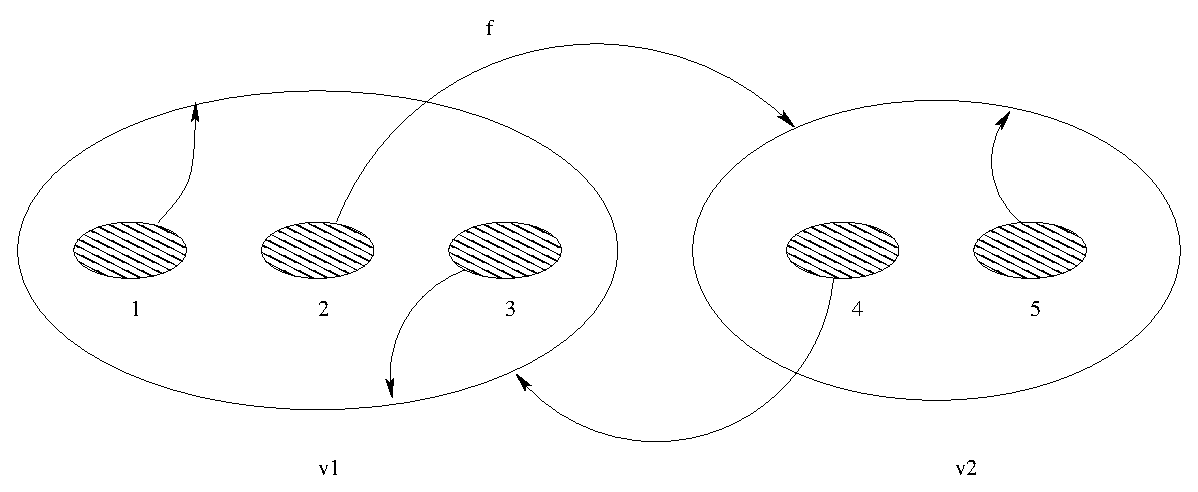
\includegraphics[scale=0.55]{cantor1.eps}
    %  note that the square brace option below is only required
    %  if you intend to produce a list of illustrations
    \caption[Shortened figure caption for the list of illustrations]
      {A Cantor repeller. Long figure captions will be indented left
      and right; short ones will be centred by default.}
    \label{cantor}
\rule[-20pt]{\textwidth}{0.6pt}
\begin{verbatim}
  \begin{figure}
    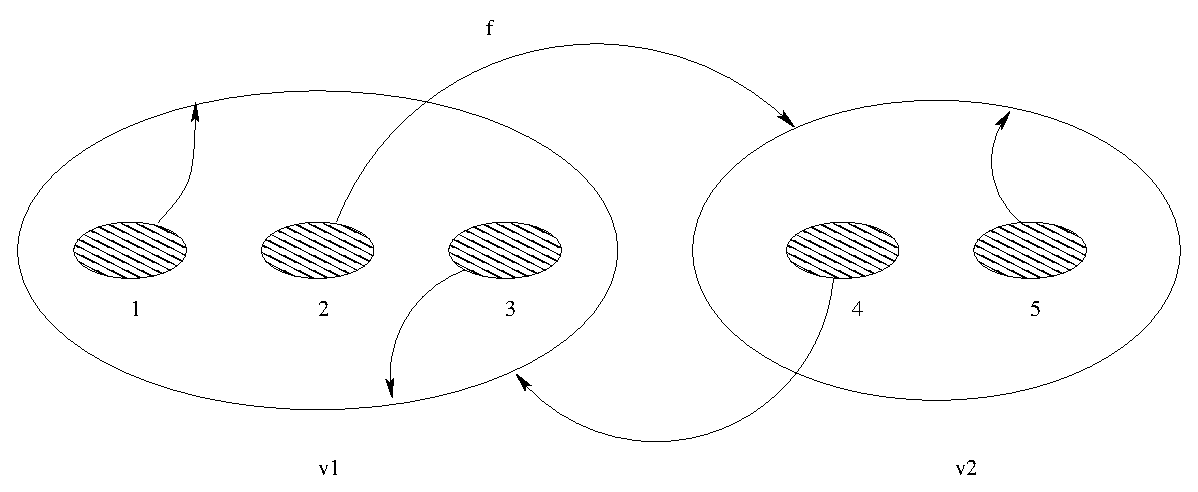
\includegraphics[scale=0.55]{cantor1.eps}
    %  note that the square brace option below is only required
    %  if you intend to produce a list of illustrations
    \caption[Shortened figure caption for the list of illustrations]
      {A Cantor repeller. Long figure captions will be indented left
      and right; short ones will be centred by default.}
    \label{cantor}
  \end{figure}
\end{verbatim}
\rule[20pt]{\textwidth}{0.5pt}
  \end{figure}

\section{Tables}

The \cambridge\ class will cope with most positioning of your tables. Table captions must be included first, the the label, then the body of the table. This is illustrated in Table~\ref{sample-table}.
  \begin{table}
    \begin{minipage}{188pt}
      %  note that the square brace option below is only required
      %  if you intend to produce a list of tables
    \caption[Shortened table caption for the list of tables]
      {Longer table captions have to be placed inside
      a minipage, otherwise they overhang the table rules.}
    \label{sample-table}
    \addtolength\tabcolsep{2pt}% to stretch columns, if required
      \begin{tabular}{@{}c@{\hspace{25pt}}ccc@{}}
        \hline \hline
        Figure\footnote{\textit{Note:} You must also use a minipage
          environment if you have footnotes.} & $hA$ & $hB$ & $hC$\\
        \hline
        1 & $\exp\left(\pi i\frac58\right)$
          & $\exp\left(\pi i\frac18\right)$ & $0$\\[3pt]
        2 & $-1$    & $\exp\left(\pi i\frac34\right)$ & $1$\\[11pt]
        3 & $-4+3i$ & $-4+3i$ & $\frac74$\\[3pt]
        4 & $-2$    & $-2$    & $\frac54 i$ \\
        \hline \hline
      \end{tabular}
    \end{minipage}
    \rule[-20pt]{\textwidth}{0.5pt}
\begin{verbatim}
  \begin{table}
    \begin{minipage}{188pt}
      %  note that the square brace option below is only required
      %  if you intend to produce a list of tables
    \caption[Shortened table caption for the list of tables]
      {Longer table captions have to be placed inside
      a minipage, otherwise they overhang the table rules.}
    \label{sample-table}
    \addtolength\tabcolsep{2pt}% to stretch columns, if required
      \begin{tabular}{@{}c@{\hspace{25pt}}ccc@{}}
        \hline \hline
        Figure\footnote{\textit{Note:} You must also use a minipage
          environment if you have footnotes.} & $hA$ & $hB$ & $hC$\\
        \hline
        1 & $\exp\left(\pi i\frac58\right)$
          & $\exp\left(\pi i\frac18\right)$ & $0$\\[3pt]
        2 & $-1$    & $\exp\left(\pi i\frac34\right)$ & $1$\\[11pt]
        3 & $-4+3i$ & $-4+3i$ & $\frac74$\\[3pt]
        4 & $-2$    & $-2$    & $\frac54 i$ \\
        \hline \hline
      \end{tabular}
    \end{minipage}
  \end{table}
\end{verbatim}
\rule[20pt]{\textwidth}{0.5pt}
  \end{table}

\subsection{My vertical rules have disappeared}

Vertical rules in tables are not \cambridge\ style, and have been automatically removed; this gives your document a truly professional look. Instead of vertical rules, we recommend the use of extra horizontal space, see Section~\ref{addhoriz}. The rules have been removed by redefining the \verb"tabular" environment. The amended definition also inserts extra vertical space above and below the horizontal rules (produced by \verb"\hline").

If you really must have them reinstated, read Section~\ref{reinstate}.

\subsection{Reinstating the vertical rules}
\label{reinstate}
Authors can revert to the standard \LaTeX\ style, if necessary. Tables will take on a rather squashed appearance, as in the \LaTeX\ book, whereby there is no added space around horizontal rules. Add the command \verb"\reinstaterules" in the preamble, and re-run your files through \LaTeX.

\subsection{There is very little space around the rules in my~table}
Tables revert to the standard, rather squashed look of standard \LaTeX\ tables for two reasons:
\begin{enumerate}
  \item you are using \verb"array.sty"; or
  \item you have chosen to reinstate vertical rules (see Section~\ref{reinstate})
\end{enumerate}
In both cases, the tabular environment is redefined.


\subsection{Adding space between columns}
\label{addhoriz}
You can add space (2pt in this example) between every column using\linebreak \verb"\addtolength\tabcolsep{2pt}". However, if you only wanted to expand the space between columns~1 and~2 to~25pt, you would do this using\linebreak  \verb"\begin{tabular}{@{}c@{\hspace{25pt}}ccc@{}}" (see Table~\ref{sample-table}).

\subsection{Adding space between rows}
If you need some form of separation between rows (for example, between rows~2 and~3 in the body of Table~\ref{sample-table}), adding \verb"[11pt]" immediately after the double backslash at the end of row~2 will add an 11pt vertical space (the equivalent of a blank line at this typesize). This is neater than adding another horizontal line.


\section{Landscape figures and tables, using rotating.sty}

Landscape figures and tables (floats) may be typeset using the \verb"rotating.sty" package. Note that the direction of rotation depends on the page number -- which requires at least two passes through \LaTeX. If we are going to know whether pages are odd or even, we need to use the \verb"\pageref" mechanism, and labels. But labels won't work unless the user has put in a caption. \textit{Beware!}

In addition to \verb"rotating.sty", you should also include \verb"floatpag.sty" and the command \verb"\rotfloatpagestyle{empty}". This combination ensures that headers and footers are removed from the float page:
\begin{verbatim}
  \usepackage{rotating}
  \usepackage{floatpag}
  \rotfloatpagestyle{empty}
\end{verbatim}
In some DVI previewers, floats may not appear rotated. If this happens, you need to convert the DVI file to PostScript or PDF.

Occasionally, when you convert a PostScript file to a PDF file, you may find that the page comes out upside-down. There will be a setting to change this. For instance, if you are using PDFCreator 0.9.7, choose the following options in this sequence:
\begin{description}
  \item Options -- Program -- PDF -- Auto-Rotate Pages: Change to `None'.
\end{description}
Other programs will have similar\vadjust{\pagebreak} procedures.


\subsection{Coding for landscape figures}

The landscape figure (Figure~\ref{sidecantor}) was typeset using the following coding:
\begin{verbatim}
  \begin{sidewaysfigure}
    \centering
    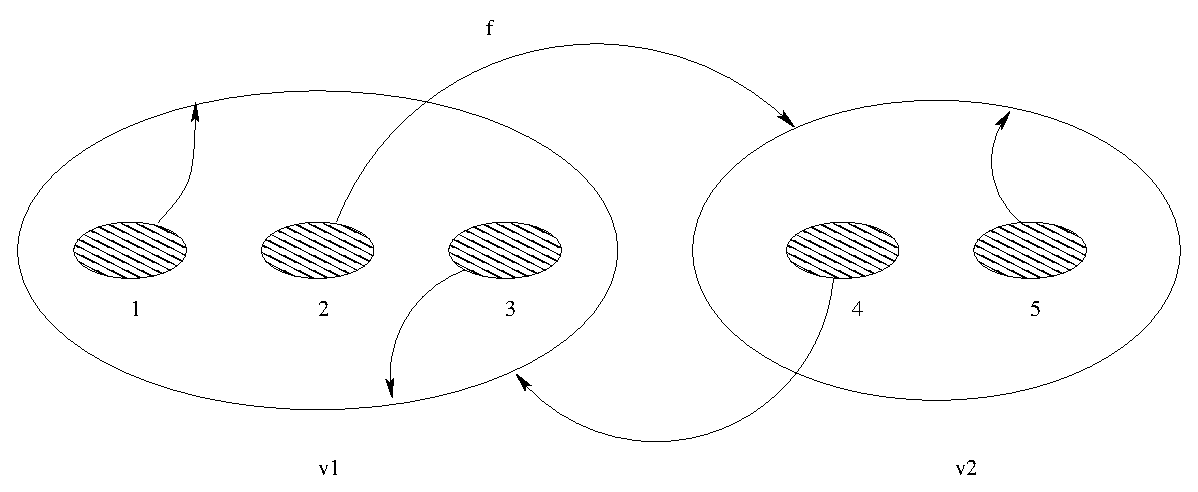
\includegraphics[scale=0.95]{cantor1.eps}
    %  note that the square brace option below is only required
    %  if you intend to produce a list of illustrations
    \caption[Landscape figure]{A Cantor repeller. Figure captions
      will be centred by default.}
    \label{sidecantor}
  \end{sidewaysfigure}
\end{verbatim}
  \begin{sidewaysfigure}
    \centering
    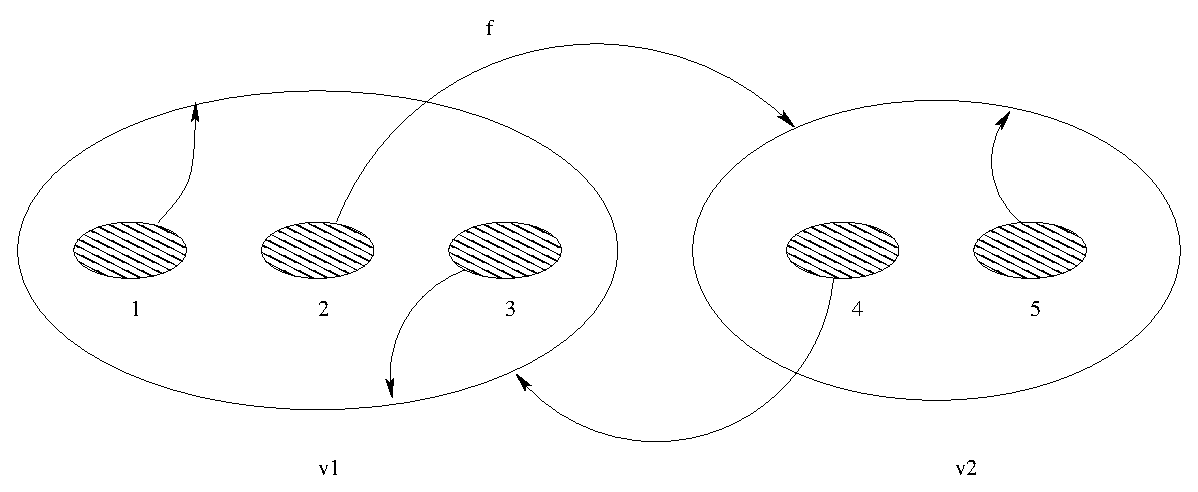
\includegraphics[scale=0.95]{cantor1.eps}
    %  note that the square brace option below is only required
    %  if you intend to produce a list of illustrations
    \caption[Landscape figure]{A Cantor repeller. Figure captions
      will be centred by default.}
    \label{sidecantor}
  \end{sidewaysfigure}



\subsection{Coding for landscape tables}

Table~\ref{sideways} has been produced using the following coding:
%
\begin{smallverbatim}
\begin{sidewaystable}
  \caption[Landscape table]{Grooved ware and beaker features, their finds and
    radiocarbon dates. For a breakdown of the pottery assemblages see
    Tables~I and~III; for the flints see Tables~II and~IV; for the animal
    bones see Table~V.}
  \label{sideways}
  \addtolength\tabcolsep{-2pt}
  \begin{tabular}{@{}lcccllccccc@{}}
  \hline\hline
  Context & Length & Breadth/  & Depth & Profile & Pottery & Flint & Animal
                                                   & Stone & Other & C14 Dates\\
  && Diameter &&&&& Bones\\[5pt]
  & m & m & m\\
  \hline\\[-5pt]
  \multicolumn{10}{@{}l}{\textbf{Grooved Ware}}\\
  784 & --   & 0.9$\phantom{0}$ &0.18  & Sloping U & P1      & $\times$46
        & $\phantom{0}$$\times$8 && $\times$2 bone & 2150 $\pm$100\,\textsc{bc}\\
  785 & --   & 1.00             &0.12   & Sloping U & P2--4  & $\times$23
                                           & $\times$21 & Hammerstone & -- & --\\
  962 & --   & 1.37             &0.20   & Sloping U & P5--6  & $\times$48
                     & $\times$57 & --& --& 1990 $\pm$80\,\textsc{bc} (Layer 4)\\
  &&&&&&&&&& 1870 $\pm$90\,\textsc{bc} (Layer 1)\\
  983 & 0.83 & 0.73             &0.25   & Stepped U & --     & $\times$18
                                & $\phantom{0}$$\times$8 & -- & Fired clay & --\\
  &&&&&&&&&&\\
  \multicolumn{10}{@{}l}{\textbf{Beaker}}\\
  552 & --   & 0.68             & 0.12  & Saucer    & P7--14 & --           & --
                                                                   & -- &-- &--\\
  790 & --   & 0.60             & 0.25  & U         & P15    & $\times$12   & --
                                                      & Quartzite-lump & -- &--\\
  794 & 2.89 & 0.75             & 0.25  & Irreg.    & P16    & $\phantom{0}$$\times$3
                                                              & -- & -- &-- &--\\
  \hline\hline
  \end{tabular}
\end{sidewaystable}
\end{smallverbatim}
%
\begin{sidewaystable}
  \caption[Landscape table]{Grooved ware and beaker features, their finds and
    radiocarbon dates. For a breakdown of the pottery assemblages see
    Tables~I and~III; for the flints see Tables~II and~IV; for the animal
    bones see Table~V.}
  \label{sideways}
  \addtolength\tabcolsep{-2pt}
  \begin{tabular}{@{}lcccllccccc@{}}
  \hline\hline
  Context & Length & Breadth/  & Depth & Profile & Pottery & Flint & Animal
                                                   & Stone & Other & C14 Dates\\
  && Diameter &&&&& Bones\\[5pt]
  & m & m & m\\
  \hline\\[-5pt]
  \multicolumn{10}{@{}l}{\textbf{Grooved Ware}}\\
  784 & --   & 0.9$\phantom{0}$ &0.18  & Sloping U & P1      & $\times$46
        & $\phantom{0}$$\times$8 && $\times$2 bone & 2150 $\pm$100\,\textsc{bc}\\
  785 & --   & 1.00             &0.12   & Sloping U & P2--4  & $\times$23
                                           & $\times$21 & Hammerstone & -- & --\\
  962 & --   & 1.37             &0.20   & Sloping U & P5--6  & $\times$48
                     & $\times$57 & --& --& 1990 $\pm$80\,\textsc{bc} (Layer 4)\\
  &&&&&&&&&& 1870 $\pm$90\,\textsc{bc} (Layer 1)\\
  983 & 0.83 & 0.73             &0.25   & Stepped U & --     & $\times$18
                                & $\phantom{0}$$\times$8 & -- & Fired clay & --\\
  &&&&&&&&&&\\
  \multicolumn{10}{@{}l}{\textbf{Beaker}}\\
  552 & --   & 0.68             & 0.12  & Saucer    & P7--14 & --           & --
                                                                   & -- &-- &--\\
  790 & --   & 0.60             & 0.25  & U         & P15    & $\times$12   & --
                                                      & Quartzite-lump & -- &--\\
  794 & 2.89 & 0.75             & 0.25  & Irreg.    & P16    & $\phantom{0}$$\times$3
                                                              & -- & -- &-- &--\\
  \hline\hline
  \end{tabular}%
\end{sidewaystable}

\endinput
\include {....}

\printindex
\end{document}
\end{verbatim}
Using the \verb|\include| command will mean that each file will have its own
\verb|.aux| file, enabling the files to be processed together or separately, by
the use of the \verb|\includeonly| command. See the \LaTeXe\ manual (pages 72--74,
210) for more information.

\section{Sectioning commands}

All chapters begin with a title and/or a number. The Cambridge University Press
style which \textsc{cmmp} implements requires minimum capitalization for all
headings; that is, only the first word and proper names take initial capital
letters -- all other words are lowercase.

For numbered chapters, use \verb|\chapter{}|. For unnumbered chapters, use
\verb|\chapter*{}|. To obtain a section head, use \verb|\section{}| (numbered)
or \verb|\section*{}| (unnumbered),  and for subsections use
\verb|\subsection{}|. In the \textsc{cmmp} style, subsections are not numbered.

\medskip
\noindent \textbf{N.B.}: the \verb|\\| command doesn't work within a
\verb|\chapter| command.

\section{Special environments}

Special environments include theorem-like environments and proofs where
the text formatting distinguishes them from the main text.

\subsection*{Theorems}

Each time you introduce a new theorem-like environment you must define it
with \verb|\newtheorem{}{}|; each environment is defined only once. All new
theorems should be defined in an external macro file which should be included
using \verb|\usepackage|.

To define a theorem-like environment, for example a corollary, type the
following:
\begin{verbatim}
\newtheorem{corollary}{Corollary}
\end{verbatim}
Here is an example of its use:
\begin{verbatim}
\begin{corollary}
This is the first corollary.
\end{corollary}
Some intervening text.
\begin{corollary}
This is the second corollary. They number automatically.
\end{corollary}
\end{verbatim}
When typeset, the above code will produce:
\newtheorem{corollary}{Corollary}
%
\begin{corollary}
This is the first corollary.
\end{corollary}
Some intervening text.
\begin{corollary}
This is the second corollary. They number automatically.
\end{corollary}
The first argument of \verb|\newtheorem| is the name of the environment as
you will refer to it with \verb|\begin{}| and \verb|\end{}|. The second
argument is the name of the environment as it will appear on the printed page.
A detailed description of the \verb|\newtheorem| command can be found in the
\LaTeXe\ manual (pages 56--57, 193--194).

\subsection*{Proofs}

For proofs, use \verb|\begin{proof}| and \verb|\end{proof}|.
\begin{verbatim}
\begin{proof}
This is the proof of the above corollary.
\end{proof}
\end{verbatim}
which looks like this in print:
\begin{proof}
This is the proof of the above corollary.
\end{proof}
\noindent A box is inserted at the end of each proof for clarity.

\section{Footnotes}

Footnotes in the \textsc{cmmp} style are numbered symbolically (with $^*$,
$^\dagger$, etc.). The footnote\footnote{An example footnote} at the bottom
of this page was keyed thus:
\begin{verbatim}
The footnote\footnote{An example footnote} at the bottom ...
\end{verbatim}
Ensure there is no space before the \verb|\| of \verb|\footnote{}|, and at
least one space after it.

\LaTeX\ imposes a limit of nine footnote symbols. If you exceed this limit
in one chapter \LaTeX\ will complain. There are two solutions to this problem:
either reduce the number of footnotes per chapter, or redefine the footnote
counter to use Arabic numbers.

\noindent e.g.
\begin{verbatim}
\renewcommand{\thefootnote}{\arabic{footnote}}
\end{verbatim}
The above code needs to be placed in the main input file, before the
\verb|\begin{document}|, or at the top of each chapter file. You should not
mix the style of footnotes within your book. Use one style or the other.

\section{Displayed equations}

There are two types of single line displayed equations, numbered and
unnumbered. Unnumbered equations can be obtained by the use of
\verb|\begin| and \verb|\end{displaymath}|. For numbered equations use
\verb|\begin| and \verb|\end{equation}|.

\noindent e.g.
\begin{verbatim}
\begin{displaymath}
x + 4 = 24
\end{displaymath}
and
\begin{equation}
x + 2 - 5 = 36
\end{equation}
\end{verbatim}
which produces
\begin{displaymath}
x + 4 = 24
\end{displaymath}
and
\begin{equation}
x + 2 - 5 = 36
\end{equation}
For unnumbered multi-line equations, use \verb|\begin| and
\verb|\end{eqnarray*}| and for numbered multi-line
equations use \verb|\begin| and \verb|\end{eqnarray}|

\noindent e.g.
\begin{verbatim}
\begin{eqnarray*}
x & = & 4 + 2 + y\\
  & = & 3 - 8 - z
\end{eqnarray*}
\end{verbatim}

\begin{verbatim}
\begin{eqnarray}
x & = & 4 + 2 + y\\
  & = & 3 - 8 - z
\end{eqnarray}
\end{verbatim}
which produces
\begin{eqnarray*}
x & = & 4 + 2 + y\\
  & = & 3 - 8 - z
\end{eqnarray*}

\begin{eqnarray}
x & = & 4 + 2 + y\nonumber\\
  & = & 3 - 8 - z
\end{eqnarray}
In addition, a new environment called \verb|ceqnarray| centres the rows of
a multi-line formula. It is used in the following way:
\begin{verbatim}
\begin{ceqnarray}
u,v  =  -v,u\\
fu,gv  =  fg u,v + fu(g)v - gv(f)u\\
o  =  u,[v,w] + w,[u,v] + v,[w,u]\\
w,u+v  =  w,u + w,v
\end{ceqnarray}
\end{verbatim}
which produces
\begin{ceqnarray}
u,v  =  -v,u\\
fu,gv  =  fg u,v + fu(g)v - gv(f)u\\
o  =  u,[v,w] + w,[u,v] + v,[w,u]\\
w,u+v  =  w,u + w,v
\end{ceqnarray}
Note that no ampersands (\verb|&|) are used in the \verb|ceqnarray| environment.
See the \LaTeXe\ manual for detailed instructions on how to format mathematical
equations with \LaTeX\ (pages 39-52, 187--191).

\section{Lists}

It is occasionally convenient to list a number of items in a format different
from that of the surrounding text. \textsc{cmmp} supplies several methods:
\begin{itemize}
\item Numbered lists, created using \verb|\begin| and \verb|\end{enumerate}|;
\item Unnumbered lists, created with \verb|\begin| and \verb|\end{unnum}|;
\item Bulletted lists, created with \verb|\begin| and \verb|\end{itemize}|;
\item Labelled lists, created with \verb|\begin| and \verb|\end{description}|.
\end{itemize}
The items in the lists are introduced with the \verb|\item| command.
Sublists can be created using the same commands; for example,
\begin{verbatim}
\begin{enumerate}
\item This is item one.
\item This is item two.
  \begin{enumerate}
  \item This is sub-item one.
  \end{enumerate}
\item This is item three.
  \begin{enumerate}
  \item This is another sub-item.
  \item This is another.
    \begin{enumerate}
    \item A subsub-list item.
    \end{enumerate}
  \end{enumerate}
\end{enumerate}
\end{verbatim}
which creates the following list:
\begin{enumerate}
\item This is item one.
\item This is item two.
\begin{enumerate}
\item This is sub-item one.
\end{enumerate}
\item This is item three.
\begin{enumerate}
\item This is another sub-item.
\item This is another.
\begin{enumerate}
\item A subsub-list item.
\end{enumerate}
\end{enumerate}
\end{enumerate}
It is important that the pairs of commands are nested properly. If you
misplace or forget a \verb|\end{}|, \LaTeX\ will complain.

\section{Illustrations}

The \verb|figure| environment allows you to integrate the artwork of a figure,
the caption, and its position on the page. Electronic integration is achieved by
using \verb"epsf.sty" or \verb"psfig.sty", both of which are freely available.
The \verb|figure| environment is used in the following way:
\begin{verbatim}
\begin{figure}[t]
\vspace{100pt}
\caption{This is the caption of my figure.}
\end{figure}
\end{verbatim}
%
\begin{figure}[t]
\vspace{100pt}
\caption{This is the caption of my figure.}
\end{figure}

The optional \verb|[t]| is a `location argument'. It tells \LaTeX\ to place
the figure at the top of a page. Other choices are \verb|[b]| for
bottom of a page; \verb|[p]| for a separate page containing no text; and
\verb|[h]| for here, the position in the text where the environment appears.

If a location argument is missing (e.g. \verb|\begin{figure}|), the default
is \verb|[tbp]|. Figures are placed at the earliest place after the point
in the text where the \verb|figure| environment occurs; a figure may not be
printed before an earlier figure and cannot violate its location argument.
Allow \LaTeX\ the greatest number of options for placing your figures, or
they might all appear at the end of your chapter. The same rules apply for
placement of tables.

Books are easier to read when the illustrations (and tables; see below) are
positioned at the tops and bottoms of the pages. This desideratum, together
with a few others, leads naturally to a fairly simple, though often
contradictory, set of rules for the positioning of floating insertions.
\begin{enumerate}
\item An illustration should be positioned after its first citation
(or call-out): preferably either at the  bottom of the page in which
it is cited on or at the top of the next page.
\item When two illustrations will fit on one page, the earlier one should
be positioned at the top of the page and the latter at the bottom.
\item A minimum of four lines of text should appear on a page with
illustrations. If less than four lines will fit on the page, it should
contain only figures (and their captions).
\item Illustrations should be positioned before the end of the section in
which they are cited and must never overlap into supplementary sections such
as bibliographies, indices, or appendices.
\item Illustrations should never be positioned on the first page of a
chapter or other major section (that is, one that begins a new right-hand
page).
\end{enumerate}
\verb|cmmp.cls| will obey most of these rules most of the time unless extreme
demands are made upon it. Badly placed figures can usually be fixed by moving
the \verb|figure| environment within the text.

Remember to leave no blank lines or space between the text and a
\verb|\begin{figure}|; it can create extra vertical space in your output.

If you have a long paragraph, you can place the \verb|figure| environment
in the centre of a paragraph; be sure to leave a blank space between
\verb|\end{figure}| and the rest of the paragraph to avoid two words printing
together with no intervening space.

Placing figures and tables correctly in a manuscript is one of the most
difficult jobs of preparing the final camera-ready copy. Before spending
lots of time positioning figures and tables, consult your editor for advice.

\section{Tables}

Tables follow the same placement rules as figures. A sample table is
inserted following this paragraph.
\begin{table}[h]
\centering
\caption{This is my table caption.}
\begin{tabular}{ccc}
\hline\hline
Zeros & Ones & Twos\\
\hline
0 & 1 & 2\\
0 & 1 & 2\\
0 & 1 & 2\\
0 & 1 & 2\\
0 & 1 & 2\\
\hline\hline
\end{tabular}
\end{table}
\newpage %%% req'd

\noindent This is how it was typed:
\begin{verbatim}
\begin{table}
\centering
\caption{This is my table caption.}
\begin{tabular}{ccc}
\hline\hline
Zeros & Ones & Twos\\
\hline
0 & 1 & 2\\
0 & 1 & 2\\
0 & 1 & 2\\
0 & 1 & 2\\
0 & 1 & 2\\
\hline\hline
\end{tabular}
\end{table}
\end{verbatim}
The CUP house style for tables is as follows:
\begin{itemize}
\item The table caption should always be above the table.
\item There should always be a horizontal double rule at the top of the
table (after the caption), and a double rule at the very end (but before
any table footnotes).
\item There should be no vertical rules.
\end{itemize}
Consult the \LaTeXe\ manual for detailed instructions regarding formatting
tables (pages 58--59, 197--200).

\section{Making a bibliography}

The bibliography begins with \verb|\begin{thebibliography}|. Each
bibliographic item should start with a \verb|\bibitem| command and should
start on a new line of its own. There are four main formats for bibliographic
items.
\begin{enumerate}
\item References to articles in journals
\item References to articles in books
\item References to books
\item References to theses and dissertations
\end{enumerate}
Examples of each are contained in the bibliography (see page~\pageref{bib}).
%%%\vadjust{\eject}

\noindent The bibliography was coded in the following way:
\begin{verbatim}
\begin{thebibliography}{4}

\bibitem{abbott}
Abbott, L.F. and Deser, S. (1982). Stability of gravity with
a cosmological constant, \textit{Nucl. Phys.} \textbf{B195},
76--96.

\bibitem{adams}
Adams, J.F. (1981). Spin (8), triality, $F_4$ and all that,
in \textit{Superspace and Supergravity}, ed. S.W.~Hawking
and M.~R\"ocek (Cambridge University Press, Cambridge).

\bibitem{arnold}
Arnol'd, V.I. (1978). \textit{Mathematical Methods of
Classical Mechanics} (Springer, New York).

\bibitem{buch}
Buchdahl, N.P. (1982). Applications of Several Complex
Variables to Twistor Theory, Oxford University
D. Phil. thesis.

\end{thebibliography}
\end{verbatim}
The standard \LaTeX\ interface has been preserved, so that Bib\TeX\ can
be used in the standard way.

\section{Making an index}

The \textsc{cmmp} document class supports the standard \LaTeX\ indexing scheme.
A detailed description on how to build an index can be found in the
\LaTeXe\ manual (pages 74--75, 211-212).

\section{Miscellaneous}

\subsection{Marginal notes}

Notes can be placed in the margin for your editor, coauthor, or yourself
with the \verb|\query| command, which works\query{This is a query} like
this:
\begin{verbatim}
works\query{This is a query} like this
\end{verbatim}
It is important that there should be no space before the \verb|\query|
command. At least one space must follow it.

\subsection{Getting the best pagebreaks}

In order to achieve the best pagebreaks, you may want to make certain
paragraphs one line longer or shorter. To make a paragraph one line longer,
use \verb|\looseness=1|; to make a paragraph one line shorter, use
\verb|\looseness=-1|. See \textit{The \TeX\ book} for details. Again before
spending lots of time on this, consult your editor for advice.

\section{Creating new commands}

To save time in keyboarding, you may define short commands for often-used
command strings. For instance, rather than typing the long
\verb|\begin| \verb|{equation}| and \verb|\end{equation}| you can type
\verb|\be| and \verb|\ee| instead, if you define them in the following way:
\begin{verbatim}
\newcommand{\be}{\begin{equation}}
\newcommand{\ee}{\end{equation}}
\end{verbatim}
Similarly, \verb|\mathcal{C}| can be replaced by \verb|\cC| (or any command
which is easy for you to remember) and \verb|\mathbf{V}| by \verb|\bV|.

If you want to reduce the number of keystrokes you have to make,
you can use  the \verb|\let}| command to abbreviate long commands.
For instance, by typing \verb|\let\bigtriangledown=\btd| you allow
either \verb|\btd| or \verb|\bigtriangledown| to be used to produce
$\bigtriangledown$.

\begin{thebibliography}{4}\label{bib}

\bibitem{abbott}
Abbott, L.F. and Deser, S. (1982). Stability of gravity with
a cosmological constant, \textit{Nucl. Phys.} \textbf{B195},
76--96.

\bibitem{adams}
Adams, J.F. (1981). Spin (8), triality, $F_4$ and all that,
in \textit{Superspace and Supergravity}, ed. S.W.~Hawking
and M.~R\"ocek (Cambridge University Press, Cambridge).

\bibitem{arnold}
Arnol'd, V.I. (1978). \textit{Mathematical Methods of
Classical Mechanics} (Springer, New York).

\bibitem{buch}
Buchdahl, N.P. (1982). Applications of Several Complex
Variables to Twistor Theory, Oxford University
D. Phil. thesis.

\end{thebibliography}

\vspace{20pt}
\hrule width 2in
\vspace{5pt}
\noindent \LaTeXe\ \textsc{cmmp} guide v1.02

\end{document}
